\documentclass[12pt, a4paper]{report}
\usepackage[utf8]{inputenc}
\usepackage[left=40mm, right=20mm, top=30mm, bottom=30mm]{geometry}
\usepackage{titlesec}
\usepackage{xparse}
\usepackage{microtype}
\usepackage{graphicx}
\usepackage{amsmath}
\usepackage{amsthm}
\usepackage{amsfonts}
\usepackage{listings}
\usepackage{bbm}
\usepackage{placeins}
\usepackage{tikz}
\usepackage{algorithm}
\usepackage{xcolor}
\usepackage{algpseudocode}
\usepackage{setspace}
\usepackage{parskip}
\usepackage[
    %backend=biber, 
    natbib=true,
    style=numeric,
    sorting=none
]{biblatex}
\usepackage{subcaption}
\usepackage{tocloft}
\usepackage{setspace}
\usepackage{multicol}
\usepackage{pgfplots} % Du brauchst dieses Package,
\pgfplotsset{compat=1.10} % diese,
\usepgfplotslibrary{fillbetween} % und diese Einstellung.

\addbibresource{bib.bib}
\titleformat{\chapter}[hang]{\Huge\bfseries}{\thechapter}{20pt}{\Huge\bfseries}
\DeclareCaptionLabelFormat{custom}{\textbf{#1 #2}}
\captionsetup{format=hang, labelformat=custom}
\graphicspath{{figures/}}
\setlength\cftbeforesecskip{-3pt}
\setlength\cftbeforechapskip{-1pt}
\setlength{\parindent}{0pt}
\setlength{\jot}{10pt}
\onehalfspacing

\renewcommand{\contentsname}{Table of Contents}
\renewcommand{\listfigurename}{\Large List of Figures \vspace{-30pt}}
\renewcommand{\listtablename}{\Large List of Tables \vspace{-30pt}}
\renewcommand{\listalgorithmname}{\Large List of Algorithms \vspace{-30pt}}

\lstdefinestyle{mystyle}{
    basicstyle=\ttfamily\tiny,
    breakatwhitespace=false,         
    breaklines=true,                 
    captionpos=b,                    
    keepspaces=true,                                                   
    showspaces=false,                
    showstringspaces=false,
    showtabs=false,                  
    tabsize=2
}

\lstset{style=mystyle}

\newtheorem{definition}{Definition}

\title{

\includegraphics[scale=0.7]{figs/logo.png} \vspace{50pt}

Optimization-inspired Barriers in Nested Sampling \vspace{20pt}

\normalsize M A S T E R ' S $\;$ T H E S I S 

in fulfillment of the requirements for the academic degree of 

Master of Science (M.Sc.)

in the study program 'Computational and Data Science' \vspace{20pt}

FRIEDRICH SCHILLER UNIVERSITY JENA 

Faculty of Mathematics and Computer Science \vspace{30pt}

submitted by Farin Lippmann 

born on the 02.02.2000 in Gera

Supervisor: Prof. Dr. Michael Habeck

}
\date{\normalsize Jena, Datum Hier}

\begin{document}
\pagenumbering{gobble}
\maketitle

\chapter*{Zusammenfassung}
Nested Sampling ist ein Algorithmus zur Anpassung von parametrischen Modellen in der Bayesschen Statistik.
Der aufwändigste Schritt im Nested Sampling ist das likelihoodbeschränkte Sampling des Priors.
Hier wird zufällig von dem Teil des Priors gezogen, der oberhalb eines bestimmten Likelihoodwerts liegt.
Standardmethoden wie Markow-Chain-Monte-Carlo-Verfahren sind hier dadurch limitiert, dass sie die Likelihood-Grenze erst dann bemerken, wenn sie bereits überschritten wurde.
In dieser Arbeit stelle ich Nested Sampling mit Barrieren vor; eine Methode, welche die Idee einer logarithmischen Barrierefunktion aus der konvexen Optimierung in Nested Sampling integriert, um das likelihoodbeschränkte Sampling des Priors gezielt zu lenken.
Dieser Ansatz erreicht %TODO: results

\chapter*{Abstract}
Nested Sampling is an algorithm for fitting Bayesian statistical models.
The most computationally expensive step in Nested Sampling involves sampling from the part of a prior distribution that lies above a certain likelihood value, called likelihood-restricted prior sampling.
Standard methods like Markov Chain Monte Carlo can be used for this step, but are limited by not noticing the likelihood-constraint-boundary until they have crossed it, causing low acceptance rates of proposals.
In this thesis, I propose Nested Sampling with Barriers, a method that incorporates the idea of a log barrier from convex optimization into Nested Sampling to guide the likelihood-restricted prior sampler.
This approach achieves %TODO: results


\clearpage
\tableofcontents
\clearpage

\chapter*{Introduction}
Bayesian models are widely used for statistical inference tasks.
They can extract information from data in a way that leads to intuitively interpretable results.
Fitting a parameterized Bayesian model comprises more than just computing a point estimate for the parameter values, as would be the case in a maximum likelihood model.
Instead, the result of Bayesian inference comprises a whole probability distribution over the parameter space, called the posterior distribution.
A distribution, as opposed to a point estimate, provides extra information about how sure we can be of the results of our inference. 

The upsides of Bayesian models come at the cost of being more difficult to fit than maximum likelihood models, especially so with increasing model complexity.
Many techniques have been developed for this purpose, the most common of which are Monte Carlo methods.
Instead of producing a parameterized version of the posterior distribution, they instead generate samples from it.
These commonly used methods (Gibbs sampling \cite{gibbs}, Metropolis Hastings \cite{metropolishastings}, Hamiltonian Monte Carlo (HMC) \cite{hmc}, Slice Sampling \cite{slice_sampling}, etc.) all come with one downside.
They focus purely on the posterior distribution of a model fit and do not compute the evidence.
The evidence is a term that comes up in Bayesian inference.
It is a useful tool that can be used to compare whole classes of models with respect to how well they fit some data.
Approaches that allow for computation of the evidence are, for example, Annealed Importance Sampling \cite{annealed_importance_sampling} and Probabilistic Integration \cite{bayesian_cubature}.
Another one is Nested Sampling, introduced by Skilling \cite{skilling}, which is the method this thesis focuses on.

Nested Sampling is a Monte Carlo method for Bayesian inference whose main objective is computing the evidence, although it can also generate posterior samples.
Nested sampling contains a step where samples have to be generated from a likelihood-restricted prior (likelihood-restricted prior sampling or LRPS).
This step is challenging \cite[9]{hmc_in_ns}, with standard Markov Chain Monte Carlo (MCMC) methods struggling to achieve high acceptance rates of proposals, because they only notice the likelihood-constraint-boundary once they have crossed it.
In this thesis, I propose a modified version of Nested Sampling which uses the idea of a log barrier from convex optimization to guide the crucial LRPS step of Nested Sampling.
This allows %TODO: results

I begin by recapping important background information about the methods and ideas this thesis is based on, including Bayesian statistics in general, the Nested Sampling algorithm and the Barrier Method for solving convex optimization problems.
Following that, using inspiration from the Barrier Method, I derive Nested Sampling with Barriers as an alternative to the standard Nested Sampling algorithm.
I then review some of the variables and parameters introduced by Nested Sampling with Barriers and analyze their effects on the algorithm.
Finally, I present the results of a benchmark where basic Nested Sampling and Nested Sampling with Barriers were run in different configurations on a set of example problems with a varying number of dimensions and modes.
\addcontentsline{toc}{chapter}{Introduction}
\pagenumbering{arabic}
\setcounter{page}{5}

\chapter{Background}
This chapter contains the background information necessary to understand the contributions of this thesis, namely Bayesian Statistics in general, Nested Sampling in particular, and the Barrier Method for convex optimization.
\section{Bayesian Statistics}
In this section, I introduce the basic principles of Bayesian statistics, including seeing probability as an extension of formal logic, generative models and Bayesian updating using Bayes' rule.

In Bayesian statistics, probability is used to model uncertainty.
Imagine we had a (possibly unfair) coin, with a certain inherent probability of landing heads (or tails) each time it is flipped.
Let us call this inherent probability of landing heads $\theta \in [0, 1]$.
If we, for example, knew that the coin was exactly fair, we could say $\theta = 0.5$.
Using the vocabulary of classical formal logic, we would say ``$\theta = 0.5$'' is true.

But since even the most accurately manufactured coin will have some microscopic asymmetries, bumps and ridges, we can never be sure of the coin's fairness.
If we are not certain whether a statement is true or false, formal logic leaves us with no options.
And if we cannot even meaningfully describe the flip of a coin, how should we expect to be able to examine complex systems like the weather, the spread of diseases, the development of ecosystems, etc.
This is where probability as an extension of formal logic can help \cite[12]{jaynes}.
We can express our knowledge of the coin's fairness by assigning a probability density to each possible value of $\theta$.
In doing so, we create a probability distribution over $\theta$.
If we knew nothing about the coin's fairness, we might assign every possible value the same probability density using a uniform distribution:
$$
    P(\theta) = 1 \quad \forall \; \theta \in [0,1]
$$
To make the example a bit more interesting, imagine we that from tossing similarly shaped coins in the past, we would assume that it would land tails more often than heads.
In this case, we might use a probability distribution like the following, which assigns lower values of $\theta$ a higher probability density:
$$
    P(\theta) = 2 \cdot (1-\theta) \quad \forall \; \theta \in [0,1]
$$
A plot of this function can be found on the left side of Figure \ref{fig:coin_example}.

By representing the coin's fairness using a parameter $\theta$, we created a simple parametric statistical model.
Statisticians would call our model generative, because by plugging $\theta$ into a Bernoulli-distribution, we can generate new samples from it, thereby simulating coin flips.
When we equip a statistical model's parameters with a probability distribution, as we did in the last paragraph, we give it what Bayesian statisticians would call a prior \cite[34]{mcelreath}.
It is called a prior since it encapsulates our beliefs about the model before we have seen any data that resulted from the process we are modeling (before we ever flipped the coin).
The name giving process of Bayesian statistics is updating our beliefs about the model's parameter values after seeing new data using Bayes' rule.
Bayes' rule prescribes how to integrate data $D$, originating from the process we are modeling, into our prior beliefs $P(\theta)$ to arrive at updated beliefs $P(\theta \, | \, D)$ (read ``probability of $\theta$ given $D$'') \cite[36]{mcelreath}.
It follows naturally from applying the product rule for probability to the joint probability of parameters and data, $P(\theta, D)$: 
\begin{align}
    P(\theta, D) &= P(\theta) \, P(D \,|\, \theta) \nonumber\\
    &= P(D) \, P(\theta \,|\, D) \nonumber\\
    P(D) \, P(\theta \,|\, D) &= P(\theta) \, P(D \,|\, \theta) \nonumber\\
    P(\theta \, | \, D) &= \frac{P(D \,|\, \theta) \; P(\theta)}{P(D)}
    \label{eq:bayes}
\end{align}

Bayes' rule (Eq. \ref{eq:bayes}) is made up of four parts.
Let us take a closer look at each of them:

\textbf{Likelihood}: Given a generative model with parameters $\theta$ in some space $\Theta$, and some data $D$ originating from the process the model is representing, we call $P(D \,|\, \theta)$ the likelihood of $\theta$, often written as $L(\theta)$.
It is the probability of the data when the model uses a certain set of parameters $\theta$.
Note that when viewed as a function of $\theta$, the likelihood is not a probability distribution, since it generally does not integrate to 1.
In the following text, the natural logarithm of the likelihood will often be abbreviated as $l(\theta) = \log(L(\theta))$.

\textbf{Prior}: Bayes' rule requires a prior distribution over the model parameters, $P(\theta)$, often written as $\pi(\theta)$.
This represents beliefs we have about the parameter values before taking the data into account, which could be results from previous experiments or qualitative knowledge about the modeled process (like in our coin example) \cite[p. 34 f.]{mcelreath}.
Priors like this may seem arbitrary or subjective, but they are required for Bayes' rule to work and have three positives:
\begin{enumerate}
    \item They provide a way to incorporate known information about the problem, which can matter especially when there is little data.
    \item With enough data, all but the most confident priors are overwhelmed and end up contributing little to the resulting posterior.
    \item Non-Bayesian methods can often be shown to be equivalent to a Bayesian inference with a certain choice of prior. \cite[36]{mcelreath} By putting our prior beliefs on display openly, they, like the model itself, become subject to the research process and scientific discussion instead of staying hidden. 
\end{enumerate}
Other authors prefer to write the prior as $P(\theta \, | \, M)$ to make explicit that it still depends on our choice of model.
I omit the conditional for the sake of less cluttered formulas, but still want to call attention to this fact.

\textbf{Evidence}: I refer to the denominator of the right side of Bayes' rule, sometimes also called marginal likelihood, average likelihood or marginal density of the data, $P(D)$, as the evidence.
It normalizes the product of prior and likelihood into a probability distribution and can also be written as follows: 
\begin{equation}
    P(\theta) = \int_\Theta P(D \,|\, \theta) \; P(\theta) \; d\theta = \int_\Theta L(\theta) \; \pi(\theta) \; d\theta
    \label{eq:evidence}
\end{equation}
Often, it is abbreviated as $Z$.
The evidence provides a measure of how well the model fits the data across all possible parameter values.
Because it averages over all parameter values, overly complex models that require a very specific combination of parameter values to do well are penalized \cite[221]{mcelreath}.
This way, the evidence provides a means to compare models that automatically accounts for overfitting. 
In general, the evidence is a huge integral and hard to compute \cite[221]{mcelreath}.
Computation of the evidence is a major focus of this thesis.

\textbf{Posterior}: The main result of most Bayesian model fitting is the posterior probability distribution over the model parameters, $P(\theta \,|\, D)$.
It represents our updated beliefs about the parameter values after having observed the data \cite[36]{mcelreath}.

Let us return to our coin example to illustrate Bayesian updating.
Say we flip the coin five times and observe the sequence H T H H H, where ``H'' means heads and ``T'' means tails.
The likelihood of any parameter value $\theta$ would then be $P(\textrm{H T H H H} \, | \, \theta)$.
For example, the likelihood of $\theta = 0.75$ would be $0.75 \cdot 0.25 \cdot 0.75 \cdot 0.75 \cdot 0.75 \approx 0.079$.
For comparison, the likelihood of $\theta = 0.25$ would be $0.25 \cdot 0.75 \cdot 0.25 \cdot 0.25 \cdot 0.25 \approx 0.0029$.
We can see how the likelihood lets us rank parameter values by how well the data supports them (see also the right side of Figure \ref{fig:coin_example}).

Now we can use Bayes' rule to generate the posterior.
For our simple, one-dimensional example we can approximate the posterior numerically by discretizing the $\theta$-space and evaluating Bayes' rule for each discrete point.
More information on how this step is done in practice follows in the next section.
For each value of $\theta$, we compute the unnormalized posterior probability $L(\theta) \cdot \pi(\theta) = P(\textrm{H T H H H} \, | \, \theta) \cdot 2 \cdot (1 - \theta)$.
We can approximate the evidence (\ref{eq:evidence}) using $Z \approx \sum_{i} L(\theta) \cdot \pi(\theta) \cdot \frac{1}{N}$, where $N$ is the number of points we discretize the $\theta$-space into.
To get our posterior values, we divide each of the unnormalized posterior probabilities by the evidence.
The posterior can be seen in the bottom image of Figure \ref{fig:coin_example}.
Note how the posterior mode lands somewhere inbetween the prior and likelihood modes.
The data updated our ideas of the coin's fairness, but did not completely override them.
If we get more data by tossing the coin a few more times, we can use the posterior we just computed as the prior of the next inference.
The more data we collect and incorporate, the more ``sure'' our posterior will be of the true value of $\theta$, becoming increasingly thin and spiky.

\begin{figure}
    \centering
    \begin{minipage}[c]{0.45\textwidth}
        \begin{tikzpicture}
            \begin{axis} [
                axis lines=center,
                xlabel=$\theta$,
                ylabel=$\pi(\theta)$,
                y label style={at={(axis description cs:-0.2, 0.5)},anchor=east},
                x label style={at={(axis description cs:0.5,-0.15)},anchor=north},
                scale=0.6
            ]
            \addplot[
                name path=A,
                domain=0:1, 
                samples=200,
                color=red
            ] { 2*(1-x) };
            \end{axis}
        \end{tikzpicture}
    \end{minipage}
    \begin{minipage}[c]{0.45\textwidth}
        \begin{tikzpicture}
            \begin{axis} [
                axis lines=center,
                xlabel=$\theta$,
                ylabel=$L(\theta)$,
                y label style={at={(axis description cs:-0.3, 0.5)},anchor=east},
                x label style={at={(axis description cs:0.5,-0.15)},anchor=north},
                scale=0.6,
                yticklabel style={
                    /pgf/number format/fixed,
                    /pgf/number format/precision=5
                },
                scaled y ticks=false
            ]
            \addplot[
                name path=A,
                domain=0:1, 
                samples=200,
                color=blue
            ] { x^4 * (1-x) };
            \end{axis}
        \end{tikzpicture}
    \end{minipage}
    \vspace{0.1cm}
    \begin{tikzpicture}
        \begin{axis} [
            axis lines=center,
            xlabel=$\theta$,
            ylabel=$P(\theta \, | \, \textrm{H T H H H})$,
            y label style={at={(axis description cs:-0.2, 0.5)},anchor=east},
            x label style={at={(axis description cs:0.5,-0.15)},anchor=north},
            yticklabel style={
                    /pgf/number format/fixed,
                    /pgf/number format/precision=5
                },
            scaled y ticks=false,
            scale=0.6
        ]
        \addplot[
            name path=A,
            domain=0:1, 
            samples=200,
            color=blue
        ] { ((x^4 * (1-x)) * (2 * (1-x))) / 0.01895};
        \end{axis}
    \end{tikzpicture}
    \caption{Prior $pi(\theta) = P(\theta)$, likelihood $L(\theta) = P(H T H H H \,|\, \theta)$ and posterior $P(\theta \,|\, H T H H H)$ of $\theta$ in the coin example with $\pi(\theta) = 2 \cdot (1-x)$ and data: H T H H H}
    \label{fig:coin_example}
\end{figure}


\section{Fitting Bayesian Models}
Having introduced Bayesian statistics and described how Bayesian inference works conceptually, let us now turn our attention to how to do it in practice.
This section briefly covers methods developed for fitting Bayesian models, starting with analytical and numerical methods, continuing to Monte Carlo methods and then Markov chain Monte Carlo methods.

\subsection{Analytical and Numerical Methods}
In some cases, the posterior can be computed analytically, yielding a parameterized probability distribution.
However, this only works for very simple models and severely limits the types of prior one can use (the prior has to be ``conjugate'' to the likelihood) \cite[39]{mcelreath}.
Another option is the one we used in the previous section, a numerical approximation utilizing a discretization of the parameter space.
This approach does not work for models with many parameters, because its computational requirements scale exponentially with the dimensionality of the parameter space.
For most real-world problems, both analytical and numerical computation of the posterior is infeasible.

\subsection{Monte Carlo Methods}
The most prevalent family of algorithms for Bayesian model fitting do not try to evaluate the posterior as a parameterized distribution, nor discretize the parameter space.
Instead, they generate samples from the posterior distribution.
These samples can then be used to approximate statistics (mean, variance, credible intervals, etc.) of the posterior distribution.
Because of their probabilistic nature, algorithms of this type are called Monte Carlo algorithms.

Generating samples from a general probability distribution is still a difficult task.
Especially for continuous distributions, where we cannot enumerate all possible values, there is no obvious way to do it \cite[358]{mckay}.
Another fact to consider is that we do not actually know the probability density function (PDF) of the distribution we want to sample from.
Because we only know the likelihood and prior, but not the evidence (see (\ref{eq:bayes})), we can only evaluate a function proportional to the posterior's density, an unnormalized version of it.
All Monte Carlo methods for Bayesian inference have to solve this problem of sampling from a distribution while only being able to evaluate an unnormalized version of its density function.

To concretize the idea of Monte Carlo, I give a brief overview of one of the simplest Monte Carlo algorithms, Rejection Sampling, in the following paragraphs.
Like most other Monte Carlo methods, Rejection Sampling makes use of a proposal distribution.
Given an unnormalized density function $\mathbf{P}(\theta)$ of the target distribution, Rejection Sampling requires a so-called proposal distribution that we can easily sample from and whose density $\mathbf{Q}(\theta)$ we can scale up using a constant $c$ to fully envelop the target density:
\begin{equation}
    c \cdot \mathbf{Q}(\theta) > \mathbf{P}(\theta) \quad \forall \, \theta \in \Theta \nonumber
\end{equation}
Then, we can generate a sample from the target distribution by sampling a $\theta^*$ from the proposal distribution and accepting the proposal with probability $\frac{\mathbf{P}(\theta^*)}{c \cdot \mathbf{Q}(\theta^*)}$.
If the proposal is not accepted, the process may be repeated until an accepted sample is found \cite[364]{mckay}.

While the simplicity of Rejection sampling is appealing, it fails in practice because
\begin{enumerate}
    \item we normally do not know the global maximum of our target distribution and thus do not know how to choose $c$, and
    \item even if we did know how to choose $c$, the fact that in high dimensional problems typically only a small fraction of the parameter space carries high posterior density forces us to scale $\mathbf{Q}$ so much everywhere else that acceptance rates plummet.
\end{enumerate}

\subsection{Markov Chain Monte Carlo Methods}
The most used algorithms in Bayesian statistics try overcome these problems by choosing a proposal distribution with dependent samples.
They are a subcategory of Monte Carlo methods called Markov chain Monte Carlo (MCMC) methods.
Each MCMC sample is dependent on its predecessor and often lands in the vicinity of it.
This allows more efficient exploration of the posterior, because once a region of high posterior density is found, its local surroundings often also carry high posterior density. 

Again, to illustrate, let us take a look at one relatively simple example algorithm, the Metropolis algorithm.
The Metropolis algorithm uses a symmetrical proposal distribution $\mathbf{Q}(\theta_{\textrm{new}} \,|\, \theta_{\textrm{old}})$.
Often, a simple normal distribution around the last sample is used.
The proposal is then accepted with probability $\frac{\mathbf{P}(\theta_{\textrm{new}})}{\mathbf{P}(\theta_{\textrm{old}})}$ \cite[p. 365f.]{mckay}.

I will not go into detail on why the Metropolis algorithm works, but I do want to at least mention the fundamentals of Markov chain Monte Carlo.
Markov chain Monte Carlo methods get their name from the fact that their samples form a Markov chain.
Markov chains are defined as a set of states $\Theta$ (in the case of Bayesian Inference these are all possible parameter values) with an initial probability distribution $P_0(\theta)$ over these states, along with a transition probability function $T: \Theta \times \Theta \rightarrow [0,1]$ assigning a probability to every transition from one state to another.
We can simulate a Markov chain by sampling an initial state $\theta_0 \sim P_0(\theta)$, then sampling the next state from the transition probability distribution $\theta_k \sim T(\theta_k \,|\, \theta_{k-1})$.
We can also analyse the probability of being in a certain state after $k$ steps \cite[372]{mckay}: 
$$
    P_k(\theta^*) = \int_{\Theta} P_{k-1}(\theta) \, T(\theta^* \,|\, \theta) \, d\theta 
$$
This also lets us define stationary distributions of Markov chains.
These are the key to using Markov chains for sampling, because once a Markov chain finds its way into a stationary distribution, it stays there.
We call $\mathcal{P}(\theta)$ a stationary distribution of a Markov chain if the probability of being in a state $\theta^*$ can be computed by integrating over the probabilites of being in any other state and transitioning to $theta^*$ \cite[372]{mckay}:
$$
    \mathcal{P}(\theta^*) = \int_{\Theta} \mathcal{P}(\theta) \, T(\theta^* \,|\, \theta) \, d\theta \quad \forall \, \theta^* \in \Theta
$$
MCMC methods focus on cleverly defining their transition probabilities in such a way that the target distribution is the only stationary distribution of the Markov chain.
That way, when the chain is sampled for long enough, it eventually produces samples from the target distribution \cite[372]{mckay}.

Now that I've touched on how Bayesian inference is normally done, I want to explain why there is room for improvement.
As covered in Section 1.1, the evidence is an immensely useful part of Bayes' formula (Equation (\ref{eq:bayes})) because it allows model comparison that accounts for overfitting.
Most MCMC methods only generate samples from the posterior, they do not compute the evidence.
Computing the evidence integral is generally a difficult task \cite[221]{mcelreath}.
Since the parameter space for real-world models is high-dimensional, with only a small fraction of this space containing meaningful posterior probability mass, numerical quadrature methods that discretize the space evenly fail.
One might think to use the modes of the posterior as a guide, since posterior density concentrates around them, but the evidence is an integral, and integration accumulates not densities, but density times volume, or mass.
In high dimensional spaces, most of the probability mass lies not at the modes, where there is high probability density, because it concentrates on very little volume.
Instead, most probability mass is found a ways out from the mode, where there is still relatively high density, but spread over magnitudes more volume.
For this reason, we cannot simply explore the posterior in a small region around the modes \cite{betancourt_talk}.
There are probabilistic integration methods like Bayesian cubature \cite{bayesian_cubature}, that estimate the evidence from a set of given MCMC samples, which by definition concentrate where there is high posterior mass.
However, this thesis focuses on a method whose main objective, from the start, is computing the evidence.


%%%%%%%%%%%%%%%%%%%%%%%%%%%%%%%%%%%%%%%%%%%%
%%%%%%%%%%%%%%%%%%%%%%%%%%%%%%%%%%%%%%%%%%%%
\section{Nested Sampling}
Nested sampling, introduced by Skilling \cite{skilling}, is an algorithm that computes the evidence of a Bayesian model while also generating samples from the posterior distribution.
In this chapter, I derive the Nested Sampling algorithm, explaining the main ideas along the way.

\FloatBarrier %TODO: READ ABOUT SEQUENTIAL MONTE CARLO IN NESTED SAMPLING FOR PHYSICAL SCIENTISTS
\subsection{From a multi- to a one-dimensional Integral}
We start by reducing the potentially multidimensional evidence integral (Equation (\ref{eq:evidence})) to a one-dimensional integral.
To this end, we first replace the likelihood in the evidence integral by its layer cake representation, a tool borrowed from measure theory \cite[26]{liebloss}.
For a quick derivation of the layer cake representation, let us define the indicator function $\mathbbm{1}_S(x)$  and the super level set $\{f \, > \, t\}$:
\begin{align*}
    \mathbbm{1}_S(x) &:= \begin{cases}
        1, & \textrm{if } x \in S \\
        0, & \textrm{otherwise}
    \end{cases} \\
    \{f \, > \, t\} &:= \{ \theta \in \Theta \, | \, f(\theta) > t \}
\end{align*}
With these definitions we rewrite $L(\theta)$ as its layer cake representation:
\begin{align*}
    L(\theta) 
    \; = \; \int_0^{L(\theta)} 1 \; d\lambda
    \; = \; \int_0^{\infty} \mathbbm{1}_{[0,L(\theta)]}(\lambda) \; d\lambda
    \; = \; \quad \int_0^{\infty} \mathbbm{1}_{\{ L \, > \, \lambda \}}(\theta) \; d\lambda 
\end{align*}
The last equality holds because the integrand is still 1 for all values of $\lambda$ that are smaller than $L(\theta)$ and 0 for all $\lambda > L(\theta)$.
Now we plug this layer cake representation of $L(\theta)$ into the evidence integral:
\begin{align}
    Z = \int_\Theta L(\theta) \, \pi(\theta) \; d\theta &= \int_{\Theta} \int_0^{\infty} \mathbbm{1}_{\{ L \, > \, \lambda \}}(\theta) \; d\lambda \; \pi(\theta) \; d\theta \nonumber\\
    &= \int_\Theta \int_0^{\infty} \mathbbm{1}_{\{ L \, > \, \lambda \}}(\theta) \, \pi(\theta) \; d\lambda \; d\theta \nonumber\\
    &= \int_0^{\infty} \int_\Theta \mathbbm{1}_{\{ L \, > \, \lambda \}}(\theta) \, \pi(\theta) \; d\theta \; d\lambda \label{eq:tonelli}\\
    &= \int_0^{\infty} \mu(\lambda) \; d\lambda
    \label{eq:integral_2}
\end{align}
We may swap the integrals in step (\ref{eq:tonelli}) thanks to Tonelli's theorem \cite[147]{measure_theory}.
With that, we have defined one of the key functions of Skilling's original paper \cite{skilling}.
$\mu$ returns, for a given likelihood-threshold $\lambda$, the amount of prior mass which exists above that likelihood threshold:
\begin{align}
\mu(\lambda) 
= \int_\Theta \mathbbm{1}_{\{ L \, > \, \lambda \}}(\theta) \, \pi(\theta) \; d\theta
= \int_{\{L \,>\, \lambda\}} \pi(\theta) \; d\theta \label{eq:mu_definition}
\end{align}
A visualization is given in Figure \ref{fig:xlambda}.

\begin{figure}
    \centering
    \begin{tikzpicture}
        \begin{axis} [
            axis lines=center,
            xticklabel=\empty,
            yticklabel=\empty,
            xtick=\empty,
            ytick=\empty,
            xlabel=$\theta$,
            x label style={at={(axis description cs:0.53,-0.02)},anchor=north}
        ]
        \addplot[
            name path=A,
            domain=-0.5:6, 
            samples=200,
            color=blue
        ] { e^(-(x-3)^2) };
        \addplot[
            name path=B,
            domain=0:6, 
            samples=200,
            color=red
        ] { 1/6 };
        \addplot[
            name path=C,
            dashed,
            domain=0:6, 
            samples=200,
            color=black
        ] { 0.8 };
        \addplot[
            name path=D,
            domain=0:6,
            opacity=0
        ] {0};
        \draw[color=black, dashed] (axis cs:2.52, 0) -- (axis cs:2.52, 0.8);
        \draw[color=black, dashed] (axis cs:3.47, 0) -- (axis cs:3.47, 0.8);
        \addplot[ 
            color=gray,
            opacity=0.2, 
            ] fill between [
                of=B and D,
                soft clip={domain=2.52:3.47} 
        ];
        \node [color=black] at (axis cs:-0.3,0.81) {$\lambda$};
        \node [color=black] at (axis cs:2.98,0.085) {$\mu(\lambda)$};
        \end{axis}
    \end{tikzpicture}
    \caption{Visualization of the relationship between a likelihood threshold $\lambda$ and the corresponding prior mass $\mu(\lambda)$ for a uniform prior (red) and a likelihood (blue).}
    \label{fig:xlambda}
\end{figure}

We will reformulate the current version of the evidence integral, (\ref{eq:integral_2}), a bit more:
\begin{align}
    Z &= \int_0^{\infty} \mu(\lambda) \; d\lambda \nonumber\\
    &= \int_0^{\infty} \mu(\lambda) \cdot 1 \; d\lambda \nonumber\\
    &\mathrel{\overset{\makebox[0pt]{\mbox{\normalfont\tiny int. by parts}}}{=}} \quad \; \; \left[\mu(\lambda) \lambda\right]_0^\infty - \int_0^\infty \mu'(\lambda)\lambda \; d\lambda \nonumber\\
    &= \underbrace{\left(\lim_{\lambda \rightarrow \infty} \mu(\lambda) \lambda\right)}_{= \, 0} - (\mu(0) \cdot 0) - \int_0^\infty \mu'(\lambda)\lambda \; d\lambda \label{eq:integral_3}\\
    &= -\int_0^\infty \mu'(\lambda)\lambda \; d\lambda \nonumber \\
    &\mathrel{\overset{\makebox[0pt]{\mbox{\normalfont\tiny int. by sub.}}}{=}} \quad \; -\int_1^0 \mu^{-1}(X) \; dX \label{eq:integral_4} \\
    &= \int_0^1 \mu^{-1}(X) \; dX \nonumber
\end{align}

Note that $\left(\lim_{\lambda \rightarrow \infty} \mu(\lambda) \lambda\right) = 0$ in (\ref{eq:integral_3}) because $\mu(\lambda)$ becomes $0$ after some finite value for $\lambda$.
The substitution used in (\ref{eq:integral_4}) is $X = \mu(\lambda)$.

Following Skilling's notation, we call the inverse of the prior mass function, $\mu^{-1}$, by the name $\mathcal{L}$.
It returns the corresponding likelihood threshold $\mathcal{L}(X)$ to a given prior mass $X \in [0,1]$.

\begin{align}
    Z = \int_0^1 \mu^{-1}(X) \; dX = \int_0^1 \mathcal{L}(X) \; dX
    \label{eq:integral_5}
\end{align}

With that, we have accomplished our goal of formulating the evidence as a one dimensional integral.
We integrate the likelihood-threshold function $\mathcal{L}$ over the prior mass values $X$.
The next section is about estimating this integral. 


\FloatBarrier
\subsection{Sampling and Sorting}

Imagine we had uniformly sampled $n$ prior mass values $X_i \in [0,1] \; \forall i \in \{1, ..., n\}$.
We could use $\mathcal{L}$ to compute their likelihood thresholds and sort them accordingly.
Since $\mathcal{L}$ is a decreasing function, this would also sort the $X_i$ in decreasing order of their own values.
For simpler notation, the $X_i$'s sorting follows their indices.
Imagine we had assigned them these indices after sorting.

\begin{align}
    \mathcal{L}(X_1)& &<& &\mathcal{L}(X_2)& &<& &\mathcal{L}(X_3) &\quad&<&   &...& &<& &\mathcal{L}(X_n) \nonumber\\
    X_1 & \quad &>& \quad &X_2 & \quad &>& \quad &X_3 &\quad&>& &...& \quad &>& \quad &X_n \label{eq:sample_ordering}
\end{align}

In the case of there being two equal likelihood thresholds, we may randomly add a very small value to one of them to artifically create an order \cite[3]{skilling}.

\begin{figure}
    \centering
    \begin{tikzpicture}
        \begin{axis} [
            axis lines=center,
            yticklabel=\empty,
            xticklabel=\empty,
            xtick=\empty,
            ytick=\empty,
            extra x ticks={0, 0.1, 0.25, 0.5, 0.85, 1},
            extra x tick labels={0, $X_4$, $X_3$, $X_2$, $X_1$, 1},
            xlabel=$X$,
            ylabel=$\mathcal{L}$,
            x label style={at={(axis description cs:0.5,-0.12)},anchor=north},
            y label style={at={(axis description cs:-0.05,.5)},rotate=90,anchor=south},
            ymin=0,
            ymax=1.2,
            xmin=0,
            xmax=1
        ]
        \addplot[
            name path=A,
            domain=0.1:0.25, 
            samples=2,
            color=black
        ] { 1 };
        \addplot[
            name path=B,
            domain=0.25:0.5, 
            samples=2,
            color=black
        ] { 0.6 };
        \addplot[
            name path=C,
            domain=0.5:0.85, 
            samples=2,
            color=black
        ] { 0.4 };
        \addplot[
            name path=D,
            domain=0.85:1, 
            samples=2,
            color=black
        ] { 0.2 };
        \draw[color=black, line width=1]{(axis cs:0.25,1) -- ( axis cs:0.25,0.6)};
        \draw[color=black, line width=1]{(axis cs:0.5,0.6) -- ( axis cs:0.5,0.4)};
        \draw[color=black, line width=1]{(axis cs:0.85,0.4) -- ( axis cs:0.85,0.2)};
        \draw[color=black, line width=1]{(axis cs:1,0.2) -- ( axis cs:1,0)};
        \draw[color=blue, line width=1]{(axis cs:0.1,1) -- ( axis cs:0.1,0)};
        \draw[color=blue, line width=1]{(axis cs:0.25,0.6) -- ( axis cs:0.25,0)};
        \draw[color=blue, line width=1]{(axis cs:0.5,0.4) -- ( axis cs:0.5,0)};
        \draw[color=blue, line width=1]{(axis cs:0.85,0.2) -- ( axis cs:0.85,0)};
        \draw (axis cs:0.1,1) node {\textbullet};
        \draw (axis cs:0.25,0.6) node {\textbullet};
        \draw (axis cs:0.5,0.4) node {\textbullet};
        \draw (axis cs:0.85,0.2) node {\textbullet};
        \addplot[
            name path=E,
            domain=0:1,
            opacity=0
        ]{0};
        \addplot[ 
            color=gray,
            opacity=0.2, 
            ] fill between [
                of=A and E,
                soft clip={domain=0.1:0.25} 
        ];
        \addplot[ 
            color=gray,
            opacity=0.2, 
            ] fill between [
                of=B and E,
                soft clip={domain=0.25:0.5} 
        ];
        \addplot[ 
            color=gray,
            opacity=0.2, 
            ] fill between [
                of=C and E,
                soft clip={domain=0.5:0.85} 
        ];
        \addplot[ 
            color=gray,
            opacity=0.2, 
            ] fill between [
                of=D and E,
                soft clip={domain=0.85:1}
        ];
        \end{axis}
    \end{tikzpicture}
    \caption{Visualization of how the evidence integral can be approximated using prior mass samples $X_i$ sorted by their likelihoods, in this case using an upper sum. The shaded region is the approximate evidence. Based on a graphic in \cite[4]{skilling}.}
    \label{fig:integral_approximate}
\end{figure}

As can be seen in Figure \ref{fig:integral_approximate}, we can approximate our target integral using the samples in the following Riemann sum \cite[p. xvi]{measure_theory}:
\begin{align}
    \int_0^1 \mathcal{L}(X) \, dX &\approx \sum_{i=1}^{n} \mathcal{L}(X_i) \cdot (X_{i-1} - X_{i}) \nonumber\\
    &\approx \sum_{i=1}^{n} \mathcal{L}(X_i) \cdot \Delta X_i \label{eq:approx_evidence}
\end{align}
where $\Delta X_i = X_{i-1} - X_{i}$ is called the prior mass shell of $X_i$, and we insert $X_0 = 1$.
Sadly, we cannot actually compute $\mathcal{L}(X)$, so prior mass samples do not help us.
We have to find another way of obtaining the terms that make up our evidence approximation in (\ref{eq:approx_evidence}).

Instead of sampling prior masses directly, we may instead sample $\theta_1, ..., \theta_n$ from the prior.
We can prove that their corresponding prior masses are uniformly distributed.

\FloatBarrier
\hrule \vspace{-0.45cm} %TODO: CHECK THAT THERE IS NO PAGE BREAK HERE
\subsubsection{Proof: Prior Masses of Prior Samples are Uniformly Distributed}
Let $\mathbb{T}$ be a random variable with the PDF $f_{\mathbb{T}}(\theta) = \pi(\theta)$; it represents samples from our prior.
Let $\mathbb{L} = L(\mathbb{T})$ and $\mathbb{M} = \mu(\mathbb{L})$ also be random variables.
$\mathbb{M}$ represents the prior masses we want to prove that it follows a uniform distribution.
First, let us take a look at the distribution of the likelihoods $\mathbb{L}$.
We can derive a nice formula for its PDF by starting with its definition as a marginal of the joint density of $\mathbb{T}$ and $\mathbb{L}$:
\begin{align}
    f_\mathbb{L}(\lambda) &= \int_\Theta f_{\mathbb{L}, \mathbb{T}}(\lambda, \theta) \, d\theta \nonumber\\
    &= \int_\Theta f_{\mathbb{L} \,|\, \mathbb{T}}(\lambda \,|\, \theta) \, f_\mathbb{T}(\theta) \, d\theta \nonumber\\
    &= \int_\Theta f_{\mathbb{L} \,|\, \mathbb{T}}(\lambda \,|\, \theta) \, \pi(\theta) \, d\theta \label{eq:L_integral}
\end{align}
Because $\mathbb{L}$ is a deterministic function of $\mathbb{T}$, the conditional density $f_{\mathbb{L} \,|\, \mathbb{T}}(\lambda \,|\, \theta)$ has to have $L(\theta)$ as the only possible outcome.
This can be modeled using the Dirac delta function $\delta(x)$, which is defined to have the following property:
\begin{equation}
    \int_0^\infty f(x) \, \delta(x - y) \, dx = f(y), \label{eq:dirac_delta_property}
\end{equation}
and can informally be imagined as being zero everywhere expect at $x=0$, where it has an infinitely large spike \cite[600]{mckay}.
Modeling $f_{\mathbb{L} \,|\, \mathbb{T}}(\lambda \,|\, \theta) = \delta(\lambda - L(\theta))$, we can plug the result into (\ref{eq:L_integral}):
\begin{equation*}
    f_\mathbb{L}(\lambda) = \int_\Theta \delta(\lambda - L(\theta)) \, \pi(\theta) \, d\theta,
\end{equation*}
and plug this representation of the PDF of $\mathbb{L}$ into the formula for its cumulative distribution function (CDF):
\begin{align}
    F_\mathbb{L}(\lambda) &= \int_0^\lambda f_\mathbb{L}(\lambda') \, d\lambda' \nonumber\\
    &= \int_0^\lambda \int_\Theta \pi(\theta) \, \delta(\lambda' - L(\theta)) \, d\theta \, d\lambda' \nonumber\\
    &= \int_\Theta \int_0^\lambda \pi(\theta) \, \delta(\lambda' - L(\theta)) \, d\lambda'\, d\theta \label{eq:tonelli2}\\
    &= \int_\Theta \pi(\theta) \int_0^\lambda \, \delta(\lambda' - L(\theta)) \, d\lambda' \, d\theta \nonumber\\
    &= \int_\Theta \pi(\theta) \, \mathbbm{1}_{\{L(\theta) < \lambda\}}(\theta) \, d\theta \label{eq:delta_property}\\
    &= \int_{\{L(\theta) < \lambda\}} \pi(\theta) \, d\theta \nonumber\\
    &= 1 - \mu(\lambda) \label{eq:L_cdf}
\end{align}
In step (\ref{eq:tonelli2}), we again use Tonelli's theorem to swap the order of the integrals \cite[147]{measure_theory}.
Step (\ref{eq:delta_property}) uses the main property of the Dirac delta function from (\ref{eq:dirac_delta_property}).
The integral is 1 as long as the spike of the delta function (which is in this case shifted to be at $L(\theta)$) is inside the integral's bounds.
Lastly, in step (\ref{eq:L_cdf}) we recognize the definition of $\mu$ from (\ref{eq:mu_definition}), only with a flipped inequality sign in the super level set.

The probability integral transform tells us that a random variable $\mathbb{Y} = f(\mathbb{X})$ is uniform if $f$ is the CDF of $\mathbb{X}$ \cite[54]{casellaberger}.
This, combined with (\ref{eq:L_cdf}) means that a random variable $\overline{\mathbb{M}} = 1 - \mu(\mathbb{L})$ would be uniformly distributed, since $1 - \mu(\lambda)$ is the CDF of $\mathbb{L}$.
Finally, since $\mathbb{M}$'s values are simply the values of $\overline{\mathbb{M}}$ mirrored at $m = 0.5$, $\mathbb{M}$ is also uniformly distributed.
\hfill $\qed$
\vspace{0.2cm} \hrule \vspace{0.2cm}

With that, we have the first part we need to approximate the evidence using (\ref{eq:approx_evidence}): the likelihood thresholds of prior mass samples.
This leaves the prior mass samples themselves.
We cannot compute the prior masses of our samples $\theta_1, ... ,\theta_n$, but we are able to estimate them using order statistics.

Order statistics study the distributions of random values when they are sorted.
The $i$-th order statistic represents the distribution of the $i$-th lowest value in a set of $n$ randomly drawn values.
We make use of the fact that when $n$ values are drawn from a $\textrm{Uniform}(0,1)$ distribution, the $i$-th order statistic follows a $\textrm{Beta}(i, n-i+1)$ distribution \cite[63]{computational_stats}.
As we remember from (\ref{eq:sample_ordering}), we can indirectly order our samples' prior masses if we order them by their likelihoods.
We know that the sample with the $i$-th lowest likelihood value will also have the $i$-th highest, or equally the $n-i+1$-th lowest, prior mass.
The prior mass thus follows a $\textrm{Beta}(n-i+1, i)$ distribution, and we can estimate it by either sampling from the distribution or by using its mean.

In $\theta_{i}$, we have thus obtained a likelihood value $L(\theta_{i})$ and an estimate for its prior mass $X_{i} \sim  \textrm{Beta}(n-i+1, i)$.
We could now simply sample $n$ values from the prior, compute their likelihoods and estimate their prior masses to get an estimate of the evidence according to (\ref{eq:approx_evidence}).
This would generally, however, lead to horribly inaccurate estimates.
Because the area of the sample space with high likelihood values is generally very small and away from the high prior values (where the prior samples will concentrate), finding samples with high likelihood that contribute significantly to the evidence would be difficult \cite[7]{skilling}.
The next section shows how this problem is solved in Nested Sampling.

\subsection{Introducing a Likelihood-Constraint} 
Nested sampling generates contributions to the evidence as in (\ref{eq:approx_evidence}) iteratively.
This allows us to modify how the contributions are sampled as the algorithm goes along.
Specifically, we can introduce a constraint that forces new contributions to be sampled in regions of higher likelihood.
This solves the problem of prior samples missing the regions with signifant posterior mass.

We need an ensemble of prior samples to use our strategy for estimating prior masses from the last section, so we start by drawing $n$ prior samples $\theta_1, ..., \theta_n$, we call these the live points.
Then we take the sample with the lowest likelihood, $\theta_{\textrm{min}}$ remove it from the live points and save it as a dead point.
We also use it to compute the first contribution to the evidence as in (\ref{eq:approx_evidence}), which is the product of its likelihood and an estimate of its prior mass shell.
Because $\theta_{min}$ has the smallest likelihood of all live points, it will also have the largest associated prior mass, $X_1$. 
This lets us simplify the estimate of its prior mass shell:
$$
    \Delta X_1 = X_0 - X_1 = 1 - X_1
$$
$X_1$ follows a $\textrm{Beta}(n,1)$ distribution and one of the properties of the Beta distribution is that if $\mathbb{X} = 1 - \mathbb{Y}$ and $Y \sim \textrm{Beta}(a,b)$, then $X \sim \textrm{Beta}(b,a)$ \cite[5.17.2.]{beta_dist}.
So $\Delta X_1$ follows a $\textrm{Beta}(1,n)$ distribution and we can again estimate it either by sampling or by using the mean.

The likelihood of $\theta_{min}$ becomes the likelihood-constraint $L^*$, meaning all points we sample thereafter have to have a likelihood higher than it.
Luckily, all other live points already fulfill this constraint, since we chose the one with the lowest likelihood to remove.
This means we only have to draw one new live point according to the constraint, $\theta_{\textrm{new}} \sim \pi(\theta) \, \mathbbm{1}_{\{L > L*\}}(\theta)$.
We call this step likelihood-restricted prior sampling (LRPS).
Having sampled a new live point, we again take the sample with the lowest likelihood, remove it from the live points, add its contribution to the evidence and set its likelihood as the new likelihood-constraint, etc.

To be sure that this strategy is correct, we have to show that the prior masses of these samples from the likelihood-restricted prior are still uniformly distributed; a proof of this can be found in the Appendix.
Also, the prior masses of $\theta_1, ..., \theta_n$ cannot follow a $\textrm{Beta}(i, n-i+1)$ distribution anymore, since the prior masses are now distributed uniformly on $[0,\mu(L^*)]$ instead of $[0,1]$.
However, if we call $\mu(L^*)$ the remaining prior mass, then the fraction of this mass that each drawn sample is connected to, $\frac{\mu(L(\theta))}{\mu(L^*)}$, is still uniformly distributed on $[0,1]$.
So we can get our estimate of the prior mass of a sample $\theta$ by sampling a mass fraction $f \sim \textrm{Beta}(0,1)$ and multiplying it by the remaining prior mass $\mu(L^*)$.

As the likelihood-constraint increases, the LRPS-samples will naturally come from regions of higher and higher likelihood.
This process is carried out for a given number of iterations or, more sophisticatedly, until an estimate of the remaining evidence in relation to the accumulated evidence becomes smaller than some chosen $\epsilon$.
A simple estimate of an upper bound of the remaining evidence can be made by taking the highest likelihood present in the live points and multiplying it by the remaining prior mass.
Once the algorithm terminates, the evidence is computed according to (\ref{eq:approx_evidence}), by multiplying each dead point's likelihood and estimated prior mass shell and summing over all of them.

Posterior samples can also be generated easily.
One randomly draws from the dead points, where each dead point's probability to be sampled is proportional to the product of its likelihood and its corresponding prior mass \cite[9]{nested_sampling_talk}.
In this aspect, Nested Sampling is similar to a technique called Sequential Monte Carlo, which also samples from previously generated points using weights.

Inputs to the algorithm are the prior and likelihood functions as well as the stopping threshold (or number of iterations) and the number of live points.
The stopping threshold determines how much of the evidence to accumulate, while the number of live points works like a resolution parameter.
The more live points we keep, the more likely we are to find and explore small peaks in the likelihood, making the evidence estimate more accurate.
More live points also cause the algorithm to take longer, since each evidence contribution will be associated with a smaller prior mass.
The number of iterations required to fulfill the same stopping threshold scales linearly with the number of live points.
Specifically, the run time of nested sampling can be described as $T \sim T_L \cdot n_{\textrm{live}} \cdot f_{\textrm{sampler}} \cdot \mathcal{D}_{\textrm{KL}}$, where
\begin{itemize}
    \item $T_L$ is the time required to evaluate the likelihood once
    \item $n_{\textrm{live}}$ is the number of live points
    \item $T_{\textrm{LRPS}}$ is the mean time required for the LRPS step over the course of the run
    \item $\mathcal{D}_{\textrm{KL}}$ is the Kullback-Leibler Divergence \cite[6]{kld} between prior and posterior \cite[1]{nested_sampling_talk}
\end{itemize}
See Algorithm \ref{alg:nested_sampling} for an overview of the Nested Sampling procedure and see a visualization in Figure \ref{fig:ns_eggcrate_example}.

\begin{algorithm}
    \caption[The basic Nested Sampling algorithm.]{NestedSampling ($n$, $\epsilon$, $\pi$, $L$)}
    \label{alg:nested_sampling}
    \begin{algorithmic}
        \State sample $\theta_1, ..., \theta_n$ from the prior $\pi$
        \State $live\_points \gets [ \theta_1, ..., \theta_n ]$
        \State $mass \gets 1$
        \State $dead\_points \gets [ \; ]$
        \State $Z \gets 0$
        \Repeat
            \State $L_{\textrm{min}} \gets \min_{\theta \, \in \, live\_points} L(\theta)$ 
            \State $\theta_{\textrm{min}} \gets \textrm{argmin}_{\theta \, \in \, live\_points} \, L(\theta)$
            \State remove $\theta_{\textrm{min}}$ from $live\_points$
            \State append $\theta_{\textrm{min}}$ to $dead\_points$
            \State sample $f$ from  $\textrm{Beta}(1, n)$
            \State $mass\_shell \gets mass \cdot f$
            \State $mass \gets mass - mass\_shell$
            \State $Z \gets Z + mass\_shell \cdot L_{\textrm{min}}$
            \State sample $\theta_{\textrm{new}}$ from likelihood-restricted prior $\pi(\theta) \, \mathbbm{1}_{\{L(\theta) > L^*\}}$
            \State append $\theta_{\textrm{new}}$ to $live\_points$
            \State $L_{\textrm{max}} \gets \max_{\theta \, \in \, live\_points} L(\theta)$
        \Until{$(mass \cdot L_{\textrm{max}}) / Z < \epsilon$}
        \State return $Z,\, dead\_points$
    \end{algorithmic}
\end{algorithm}

\begin{figure}
    \centering
    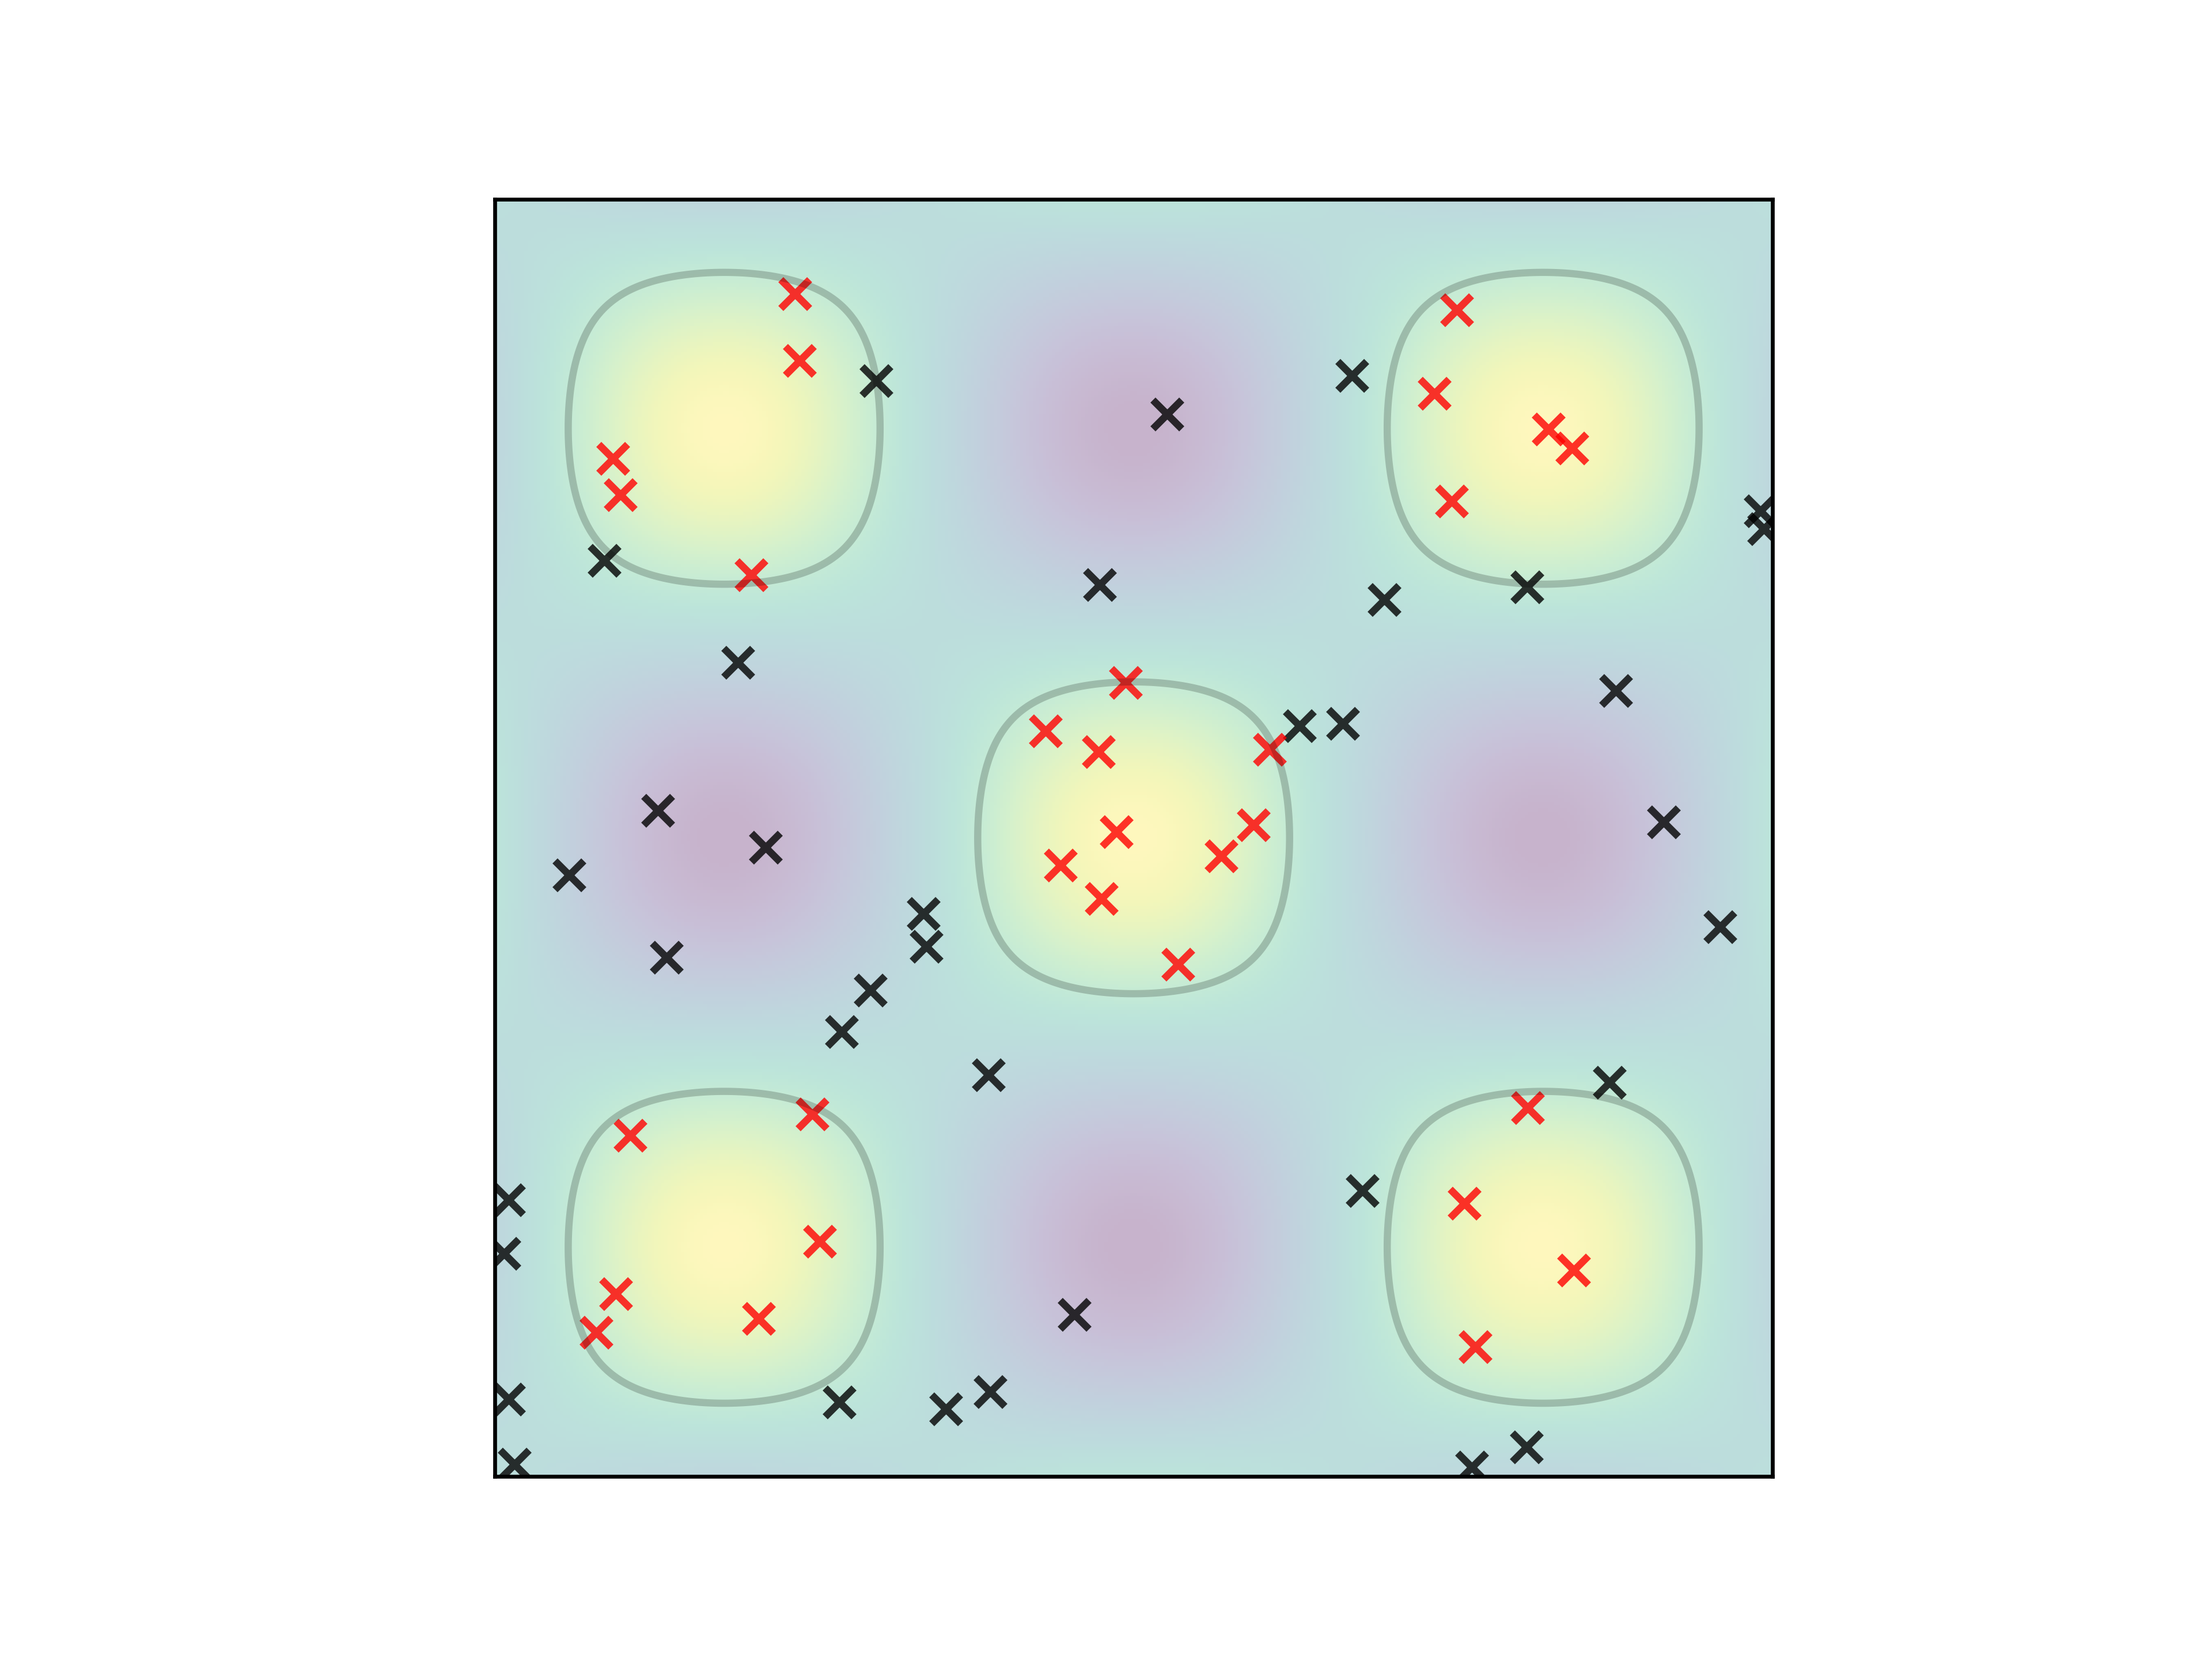
\includegraphics[trim={3cm 1cm 2.4cm 1cm}, clip, scale=0.65]{figs/ns_eggcrate_example_1.png}
    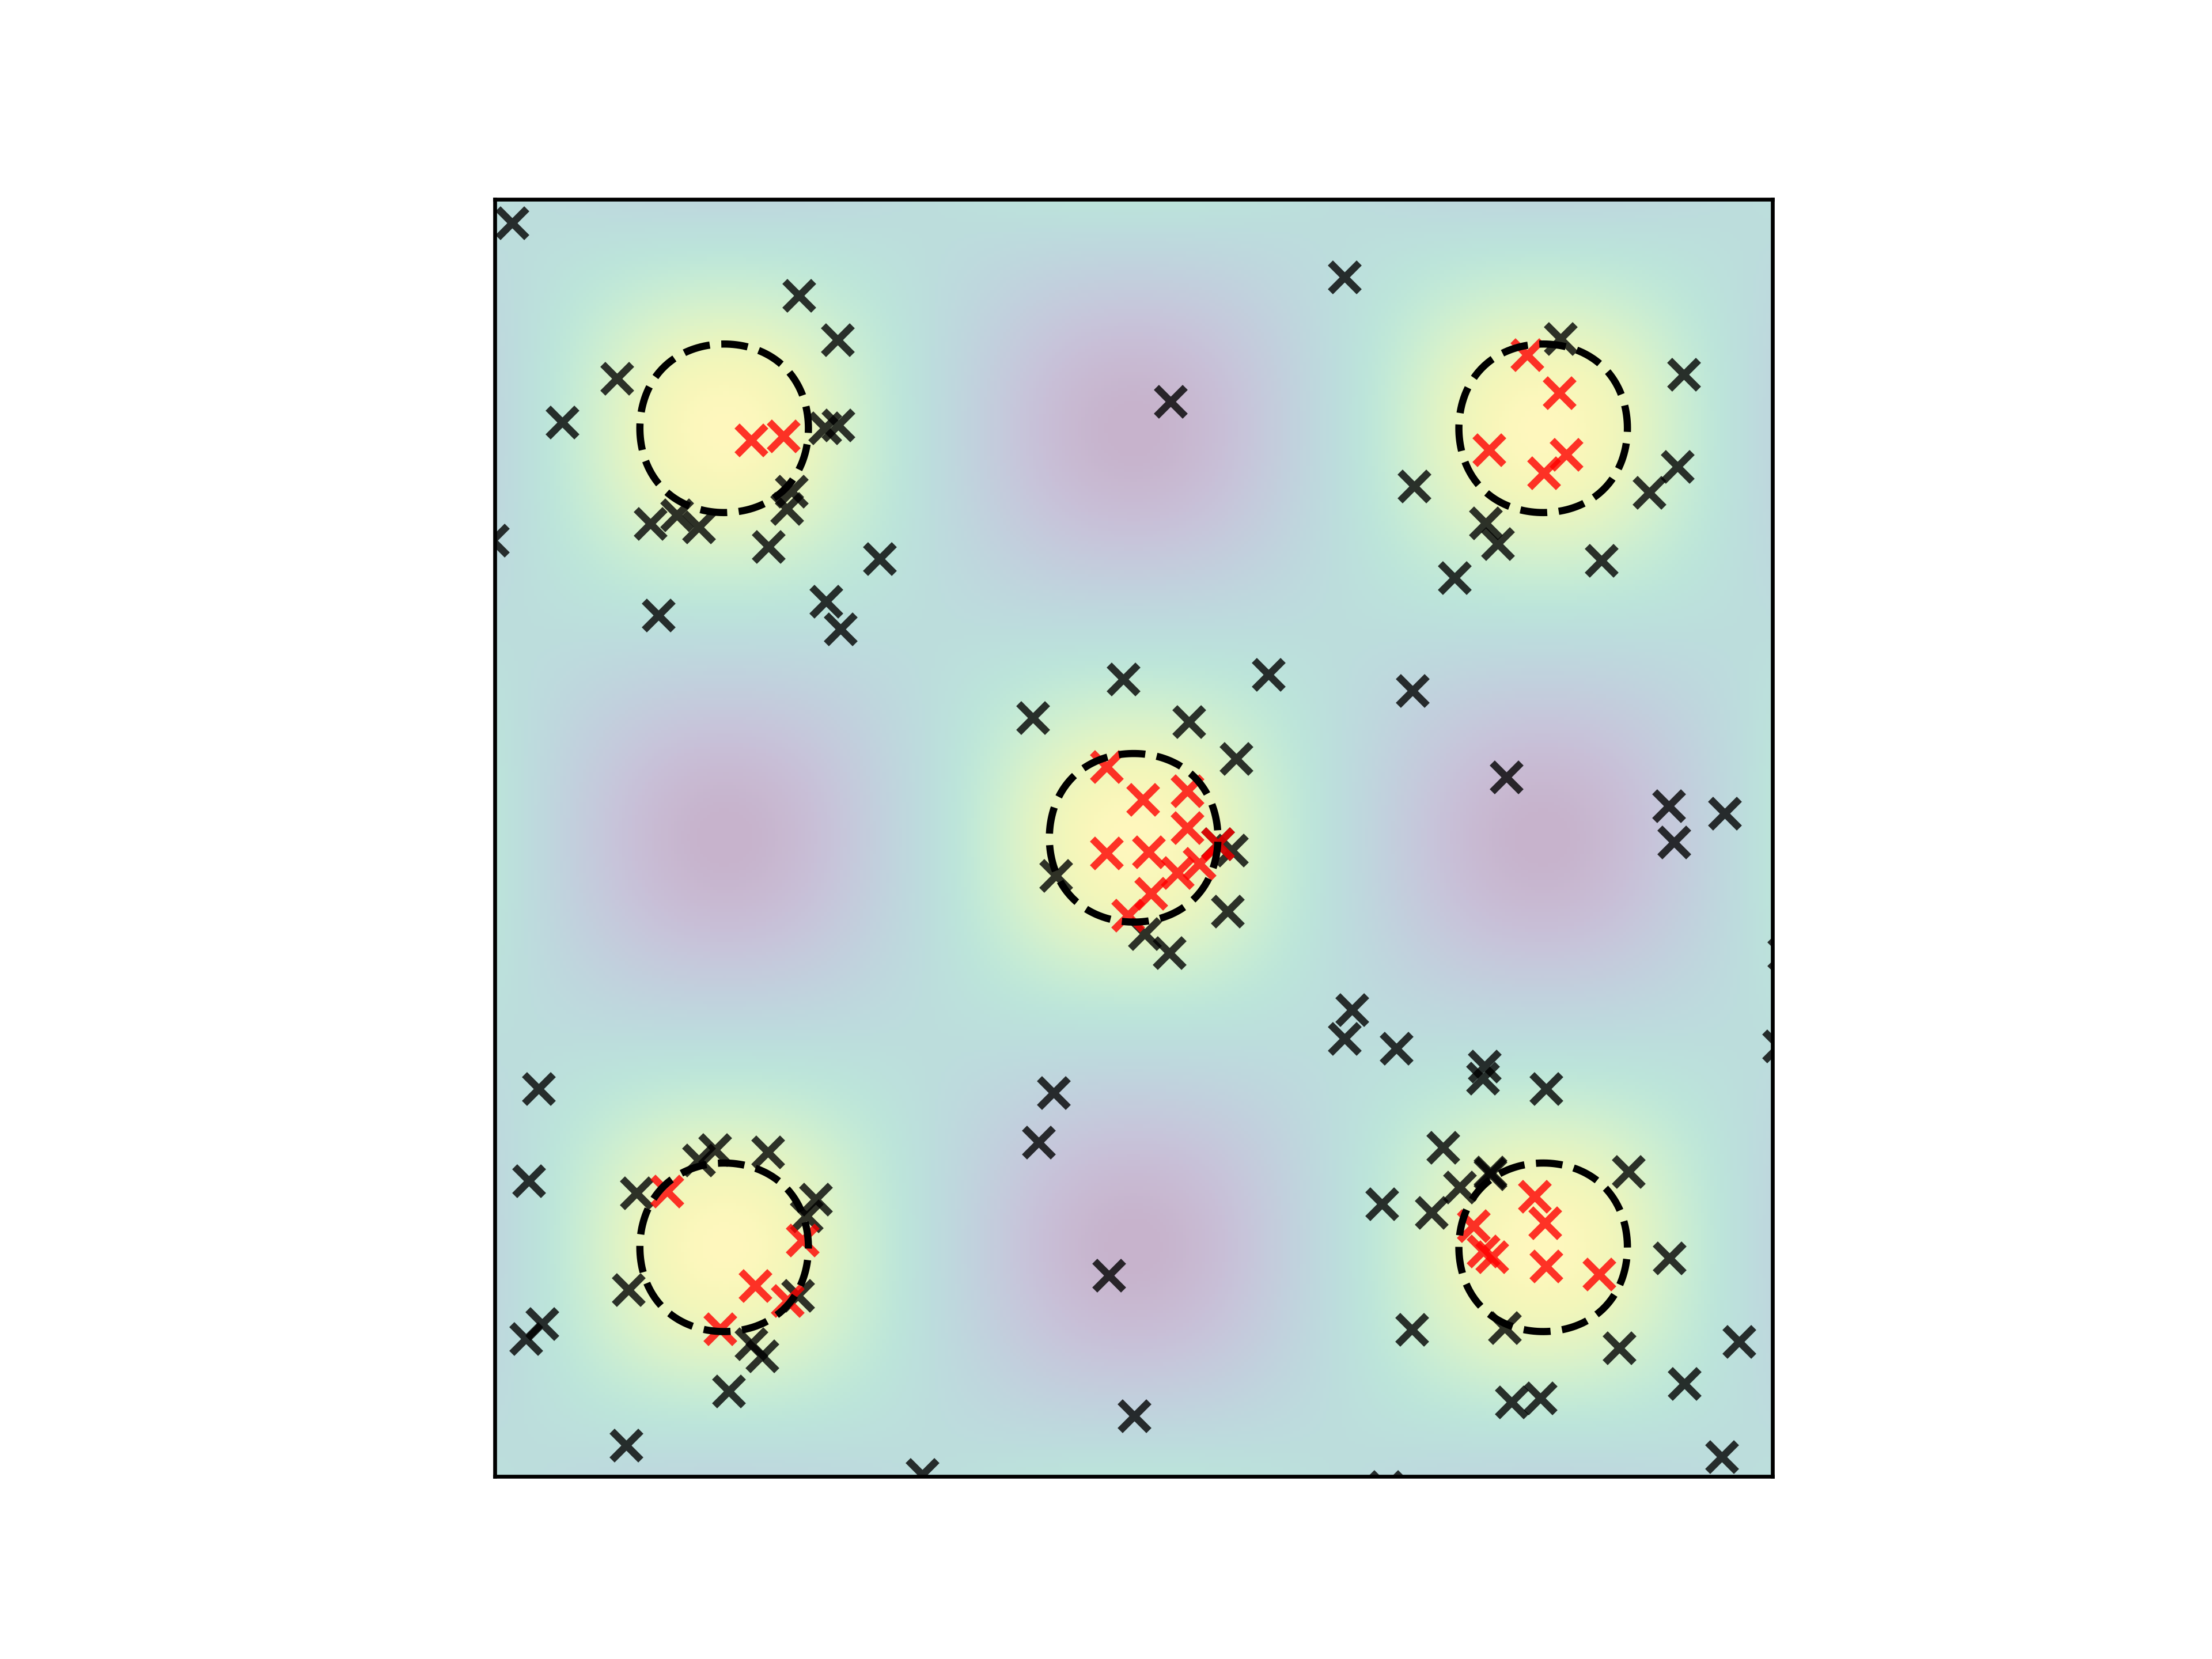
\includegraphics[trim={2.4cm 1cm 3cm 1cm}, clip, scale=0.65]{figs/ns_eggcrate_example_2.png}
    \caption{Intermediate states of two Nested Sampling runs on an eggcrate-shaped likelihood with a uniform prior. Black crosses are dead points, red crosses are live points. All live points are inside the current likelihood-constraint contour. The likelihood is visualized by the colored background, lighter colors represent higher likelihood values. The left image shows an earlier iteration than the right one, as can be seen by the lower number of dead points and the looser likelihood-constraint contours.}
    \label{fig:ns_eggcrate_example}
\end{figure}

Having explained the main ideas of Nested Sampling, let us now get into the details of the most computationally intensive and least clearly defined step of it, LRPS.

\FloatBarrier
\section{Likelihood-restricted prior sampling}
In the sampling of new points from the likelihood-restricted prior lies most of the computational work of Nested Sampling.
The original paper by Skilling provides little guidance for this step, only that "such points will usually be found by some MCMC approximation, ..." \cite[6]{skilling}
In this section, we summarize multiple ways to do LRPS while presenting their advantages and drawbacks, working our way up from the simplest methods to more complex ones.

\subsection{Rejection Sampling}
Rejection sampling is the simplest way to sample from the constrained prior.
We generate a sample from the prior, compute its likelihood and check if it satisfies the likelihood-constraint.
If it does, we accept the sample; otherwise, we reject it.

Rejection sampling is infeasible larger models due to it being terribly inefficient in higher dimensions.
The acceptance rate of the generated samples is proportional to how much of the prior mass is inside the likelihood-constraint.
Since the prior mass inside the likelihood-constraint is expected to shrink by a factor of $\frac{1}{1+n}$ (mean of the $\textrm{Beta}(1, n)$ distribution) each iteration, the acceptance rate quickly plummets, leading to most proposals being rejected.

\subsection{Discretized LRPS}
Another simple, non-MCMC method for LRPS involves discretizing the sample space into a uniform grid.
In each iteration, we randomly draw one of the grid points with likelihood higher than the constraint, with the probability of each point being drawn being proportional to its prior.

Like Rejection Sampling, this method falls short because of its lacking performance and can only be used for models with few parameters and priors with finite support.
Since the number of grid points scales exponentially with the dimensionality of the sample space, this method is hopelessly time- and memory-inefficient for problems with even a modest number of dimensions.

\subsection{Metropolis Algorithm}
The Metropolis algorithm, already sketched out in Section 1.1, is an MCMC method generating dependent samples using a proposal distribution.
The proposal distribution, often a normal distribution, creates a proposal $\theta_p$ based on the last sample $\theta$.
This proposal is then accepted with a probability $\textrm{max}\left(\frac{P(\theta_p)}{P(\theta)}, 1\right)$.
In LRPS, this process is repeated a given number of times to decorrelate the samples.
Proposals which do not satisfy the likelihood-constraint are never accepted.
Details can be seen in Algorithm \ref{alg:lrpsmetropolis}.
If the proposal distribution is not symmetric, the standard Metropolis algorithm fails, but a variant called Metropolis-Hastings can be used \cite[p. 365f.]{mckay}.
\begin{algorithm}
    \caption[Likelihood-restricted prior sampling using Metropolis.]{LRPSMetropolis ($n$, $\theta_0$, $\pi$, $\sigma$, $L$, $L^*$)}
    \label{alg:lrpsmetropolis}
    \begin{algorithmic}
        \State $\theta \gets \theta_0$
        \For{$n$ iterations}
            \State sample $\theta_p$ from $\mathcal{N}(\theta, \sigma^2)$
            \State sample $u$ from $\textrm{Uniform}(0, 1)$
            \If{$L(\theta_p) > L^*$ and $\pi(\theta_p) / \pi(\theta) > u$}
                \State $\theta \gets \theta_p$
            \EndIf
        \EndFor
        \State return $\theta$
    \end{algorithmic}
\end{algorithm}

The main advantage of the Metropolis algorithm in LRPS is its local exploration.
Since it always starts from a valid point and explores its local surroundings, its acceptance rate can be much higher than that of Rejection Sampling.
It does, however, have two major disadvantages.
Firstly, because the samples are dependent, we have to draw many intermediate samples before returning an actual sample, to allow them to decorrelate.
Secondly, since the proportion of prior space within the likelihood-constraint becomes smaller with each Nested Sampling iteration, the step size (standard deviation of the proposal distribution) required to efficiently explore the space changes continually.
This second problem can be overcome by using an adaptive step size.
A simple approach would be to decrease the step size by some factor each time a sample lands outside the likelihood-constraint while increasing it whenever a sample lands inside the constraint.
More nuanced methods for step size adaptation have been developed as well \cite{automala}.

\subsection{Hamiltonian Monte Carlo}
Hamiltonian Monte Carlo (HMC) is a widely used MCMC algorithm for Bayesian model fitting.
Normally used to sample from the posterior of a Bayesian model all on its own, we can also appropriate it for LRPS.
As the theory behind HMC is quite involved, I will only give an overview of the algorithm, not delving into the reasons for why it works.

As HMC is an MCMC method, it generates dependent samples like the Metropolis algorithm does.
However, it uses a physical analogy to find samples that are much further away from the starting point, thus decorrelating and exploring the target distribution faster.

The negative logarithm of the target distribution is viewed as representing potential energy.
One can imagine this as a hills-and-valleys landscape.
Each sample is viewed as a movable particle in this space.
Starting with a sample, a random, normally distributed vector is drawn.
This vector represents a momentum that the sample particle has.
The path of the particle across the landscape with its given starting momentum is then simulated using a special type of solver for partial differential equations called a symplectic integrator.
At an arbitrarily chosen point of time, the particle is stopped.
The resulting position of the sample is then treated like a Metropolis proposal and accepted with a probability based on the ratio of probability values of the proposal and the last sample.
A visualization of this process can be seen in Figure \ref{fig:hmc_example}.
Betancourt provides a thorough explanation of HMC with solid theoretical foundations in \cite{hmc}.

\begin{figure}
    \centering
    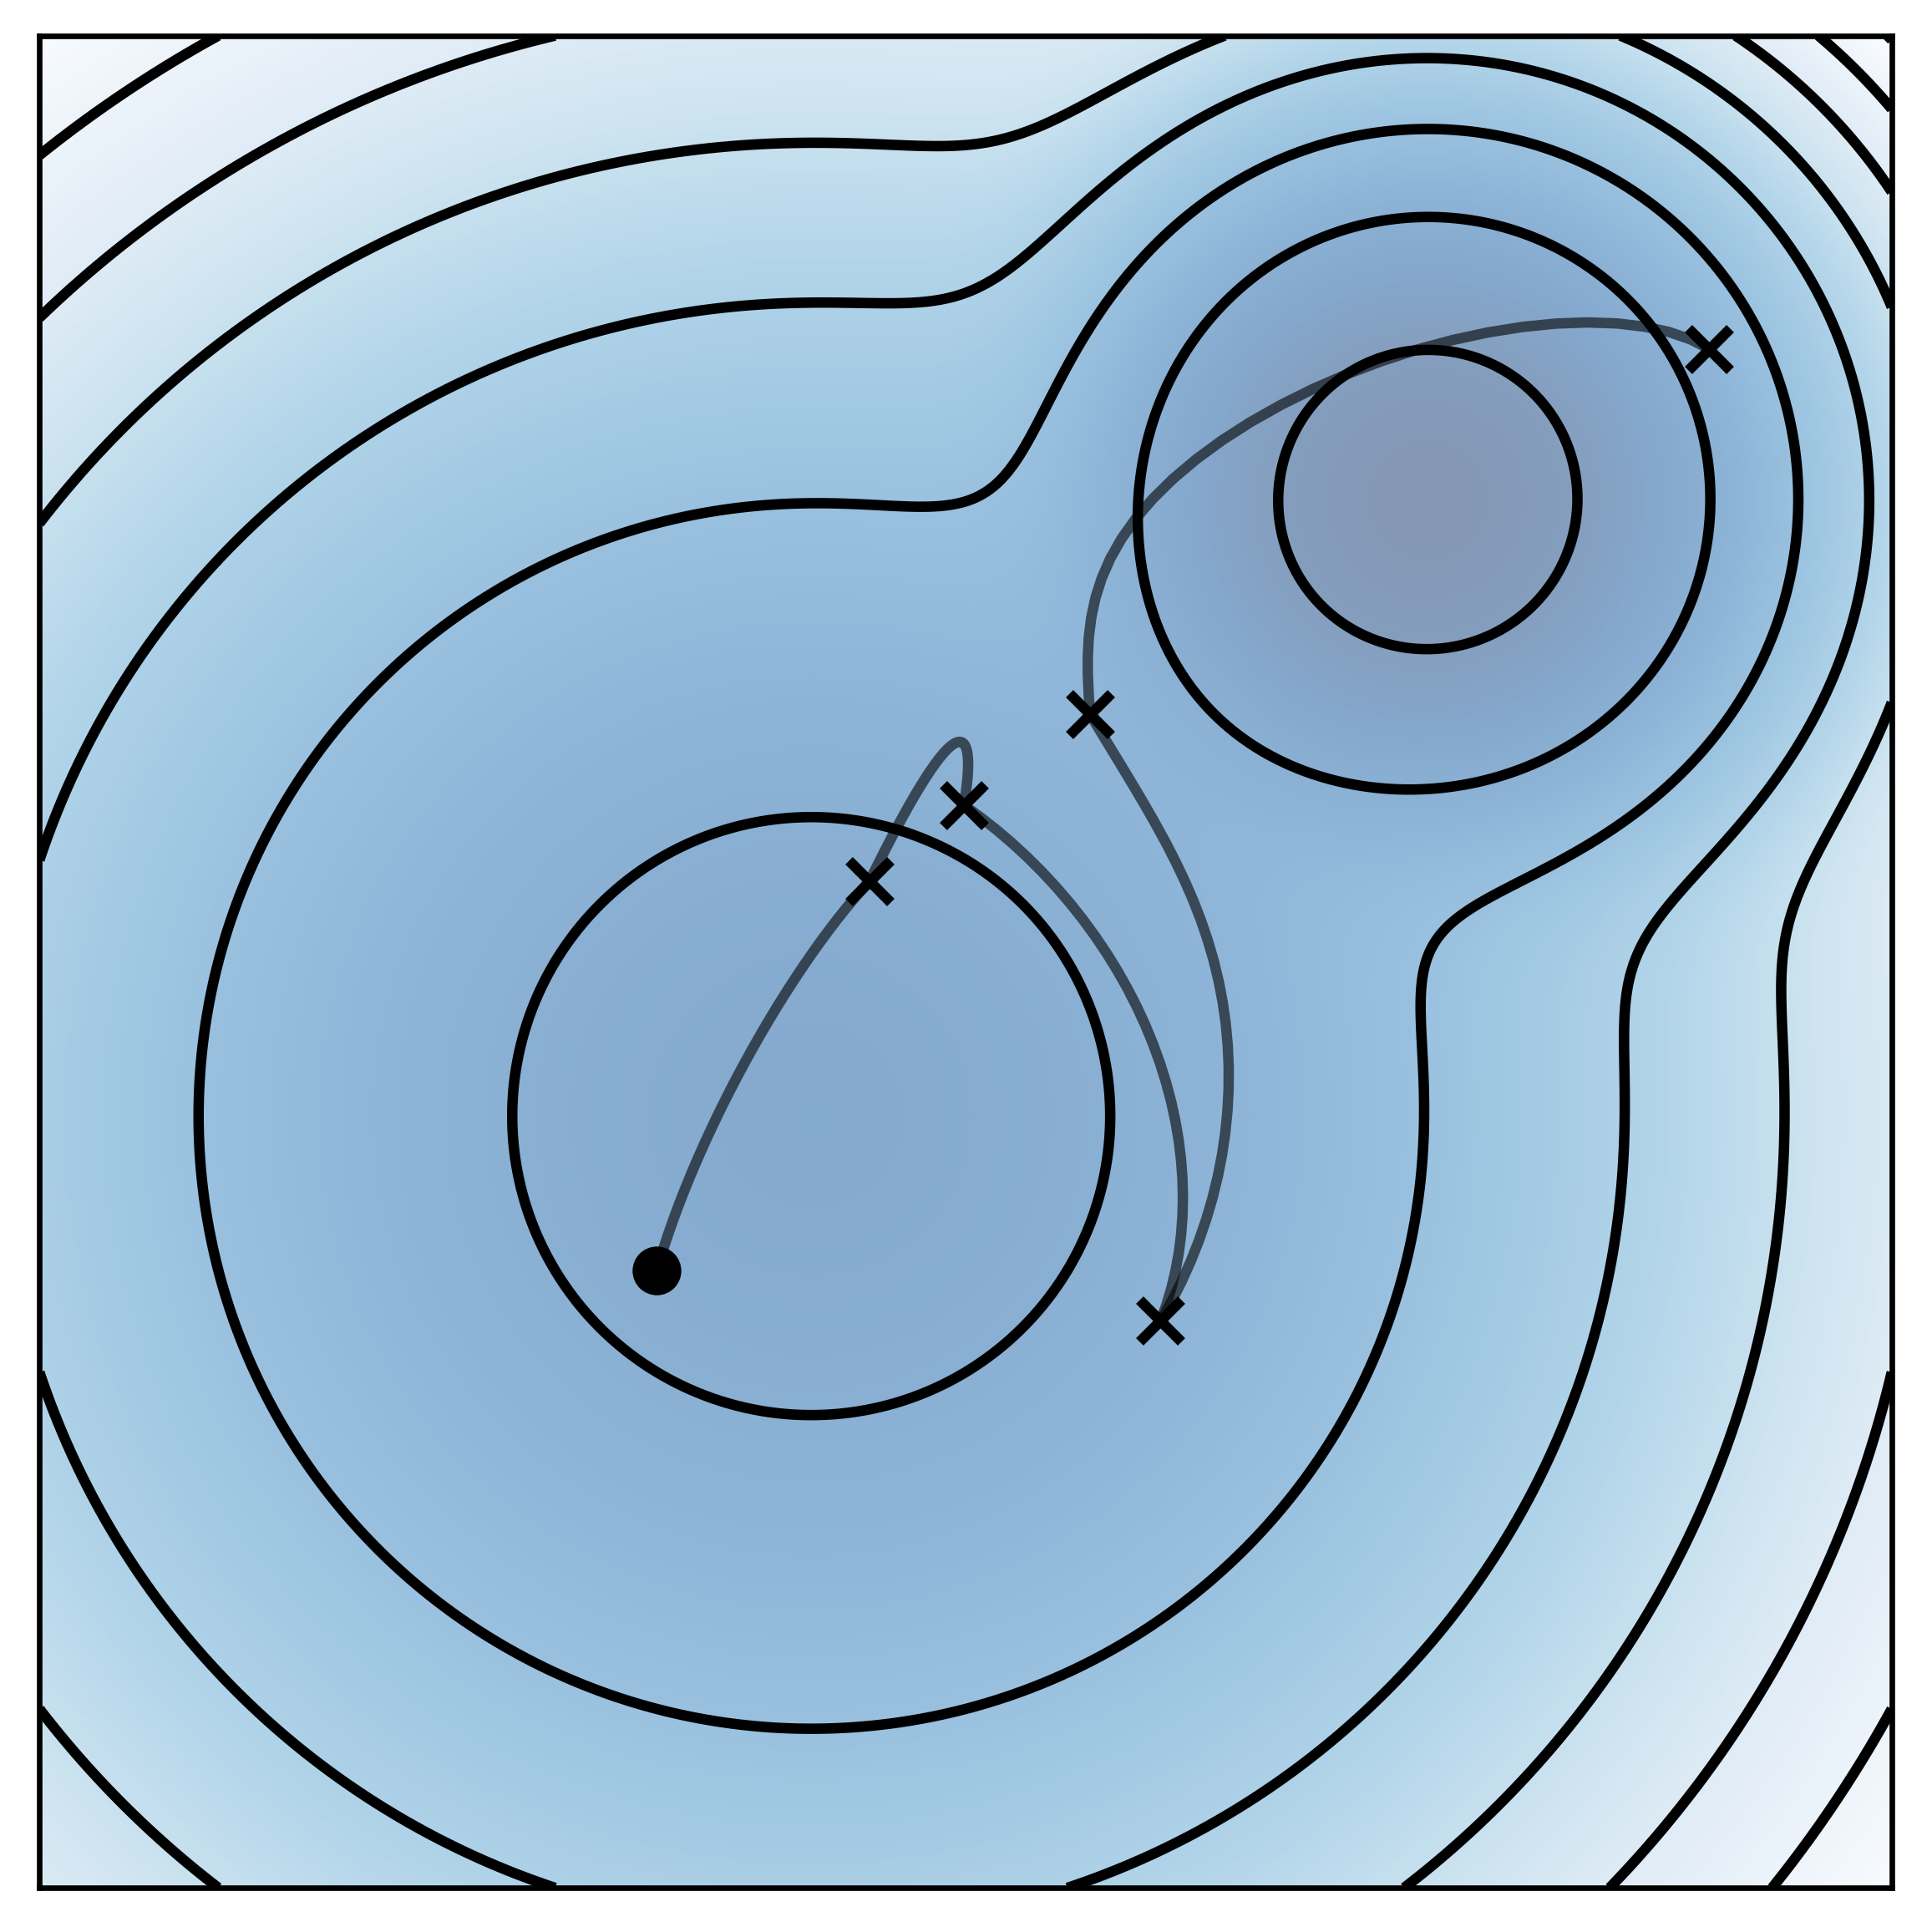
\includegraphics[scale=0.8]{figs/hmc_example.png}
    \caption{Visualization of HMC in a two-dimensional sample space. Contour lines and shading indicate the negative log probability of the target distribution (a mixture of two Gaussians). The dot is the starting point and each cross is a sampled point.}
    \label{fig:hmc_example}
\end{figure}

HMC can be adapted for LRPS.
In this case, the negative logarithm of the prior provides the landscape for the particles to move around in.
The starting spot for a particle is always chosen to satisfy the likelihood-constraint (e.g. by choosing one of the live points).
HMC evolves the particle through the prior space to generate a new sample.
The main adaptation made is when the particle hits the likelihood-constraint barrier.
In this case, it is reflected off the barrier to stay inside the valid region.
This adaptation of HMC was introduced by Betancourt in \cite{hmc_in_ns}.

Like the Metropolis Algorithm, HMC for LRPS requires an adaptive step size.
Without it, the tight likelihood constraint boundary during the later iterations of Nested would lead to degenrate behavior as HMC reflects with every integration step.
This is especially bad since the likelihood gradient used for reflection is calculated at the end of the integration step that lands outside of the likelihood constraint.
If the step size is very large in relation to the valid sampling area, the gradient will be calculated far away from the actual constraint boundary, leading to inaccurate reflection.
See the visualization in Figure \ref{fig:hmc_reflection_example}.

\begin{figure}
    \centering
    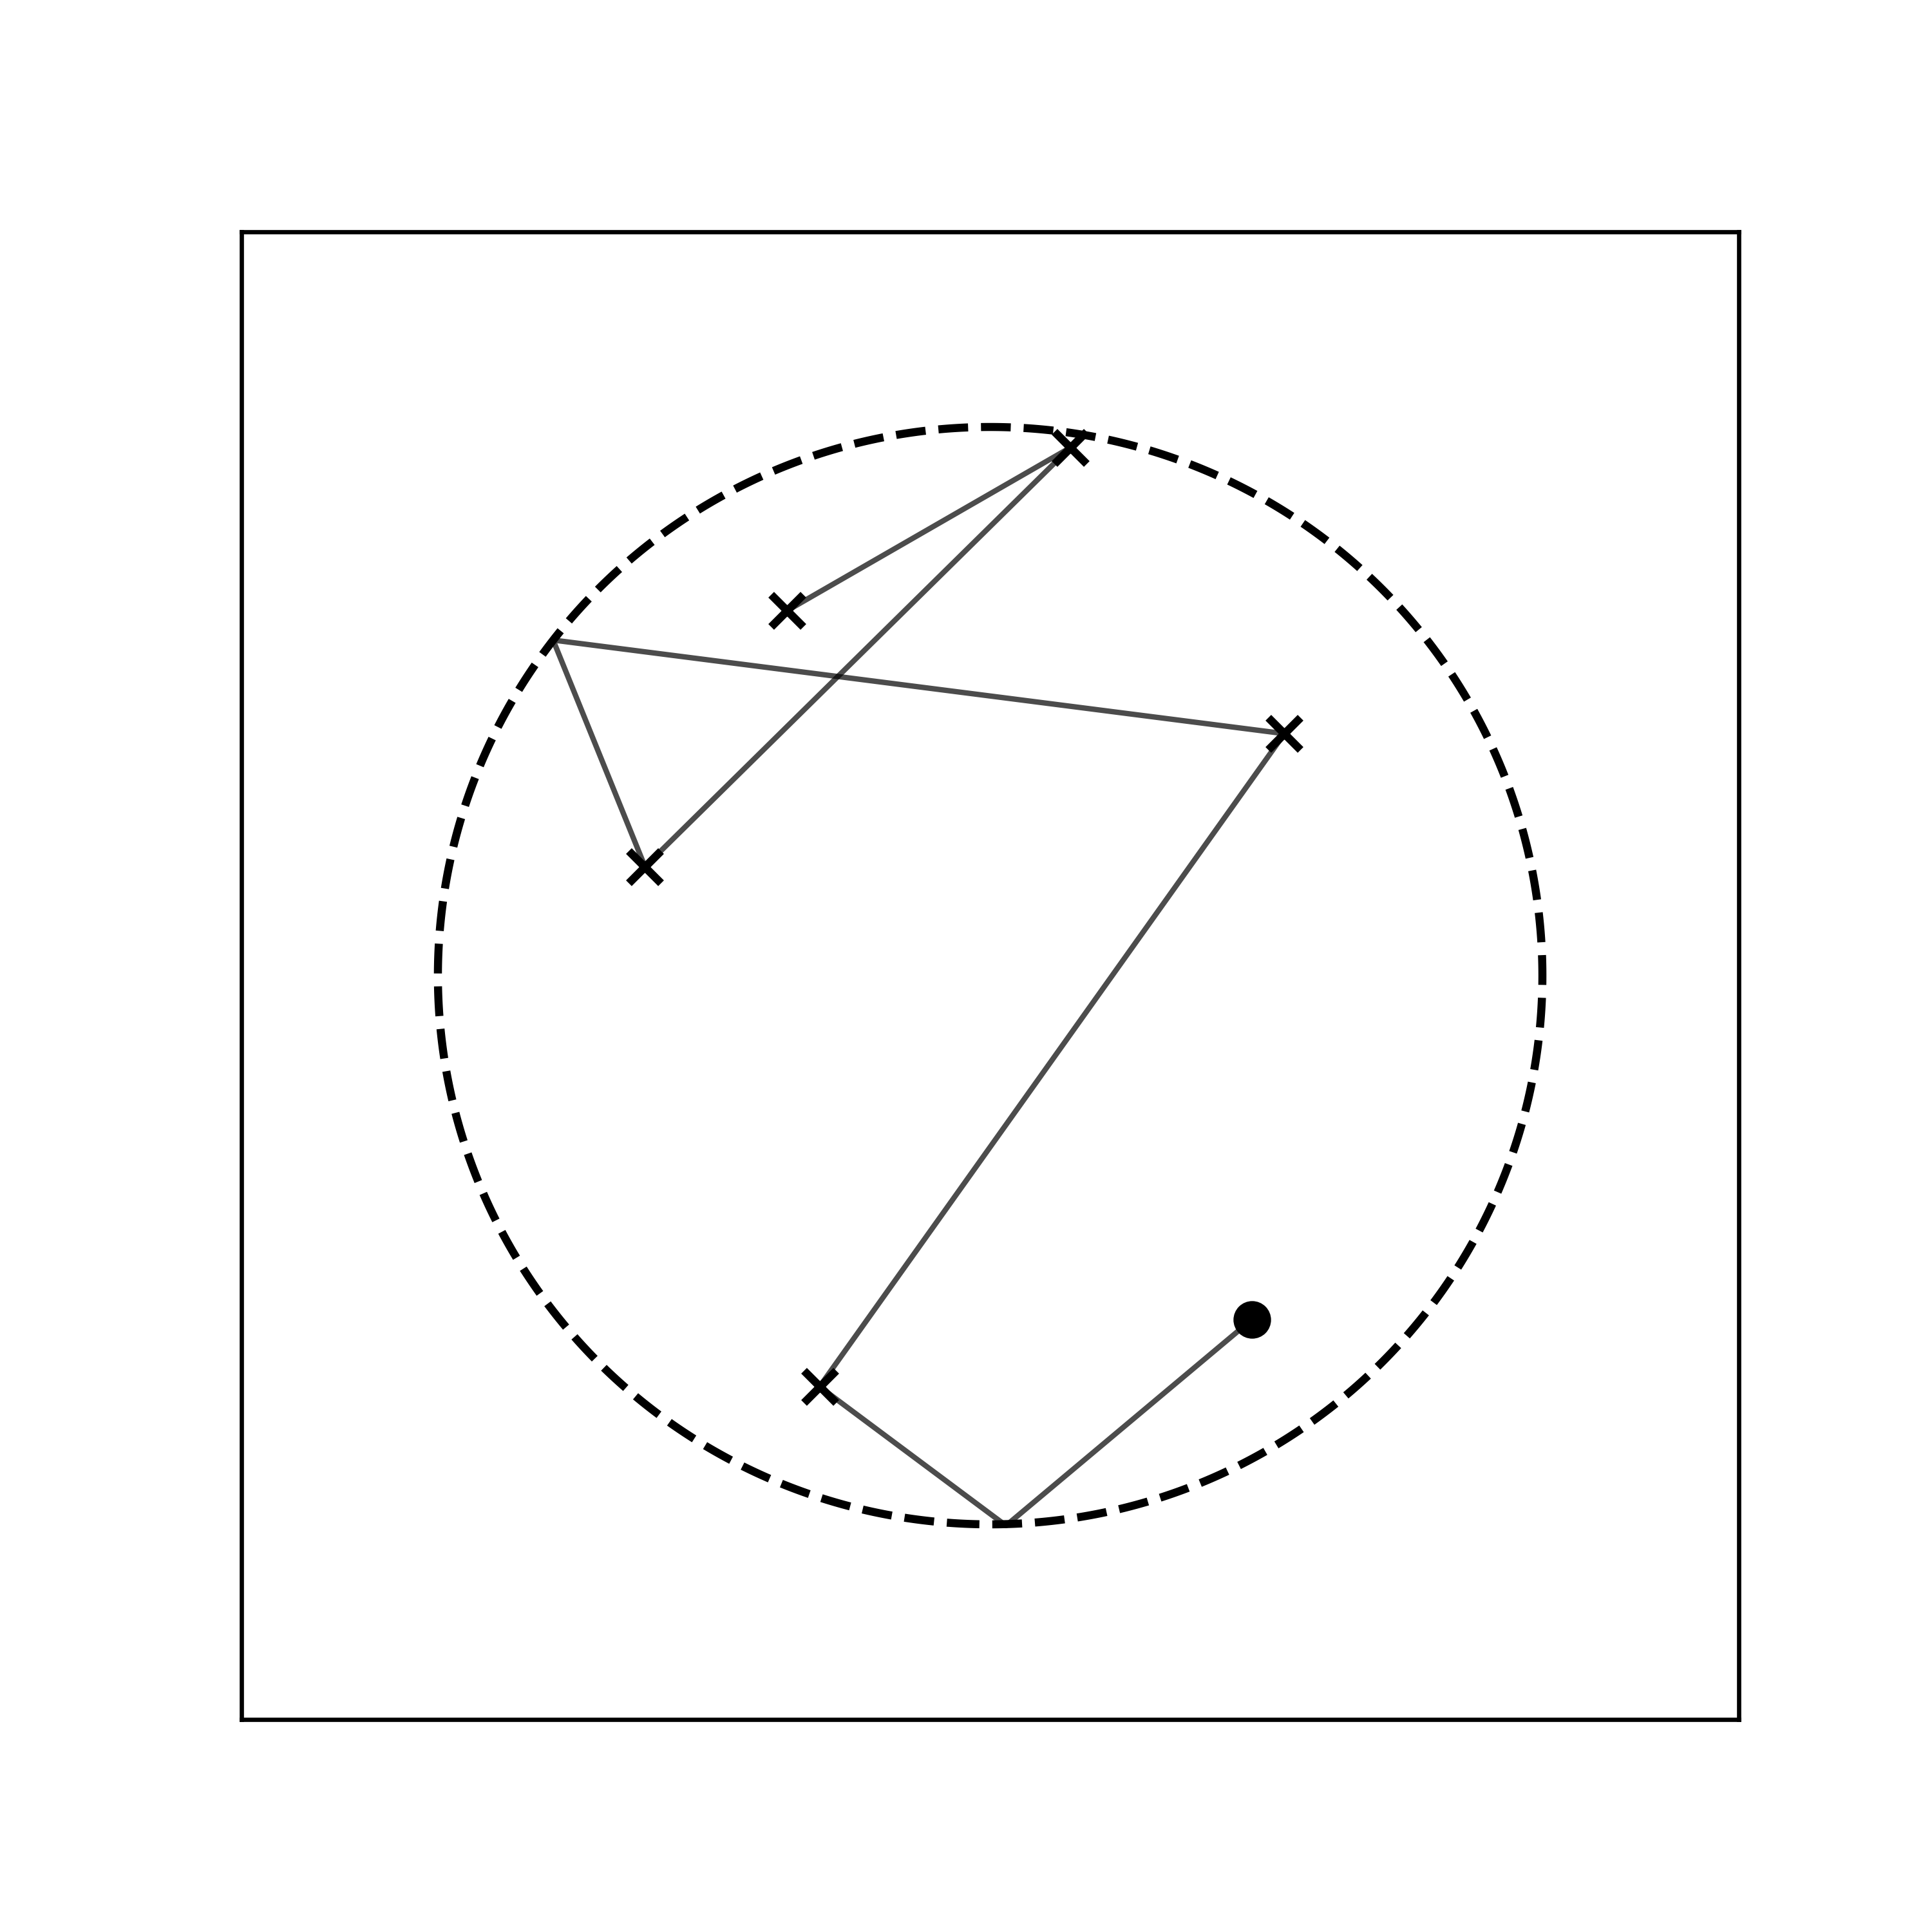
\includegraphics[scale=0.45]{figs/hmc_reflection_example.png}
    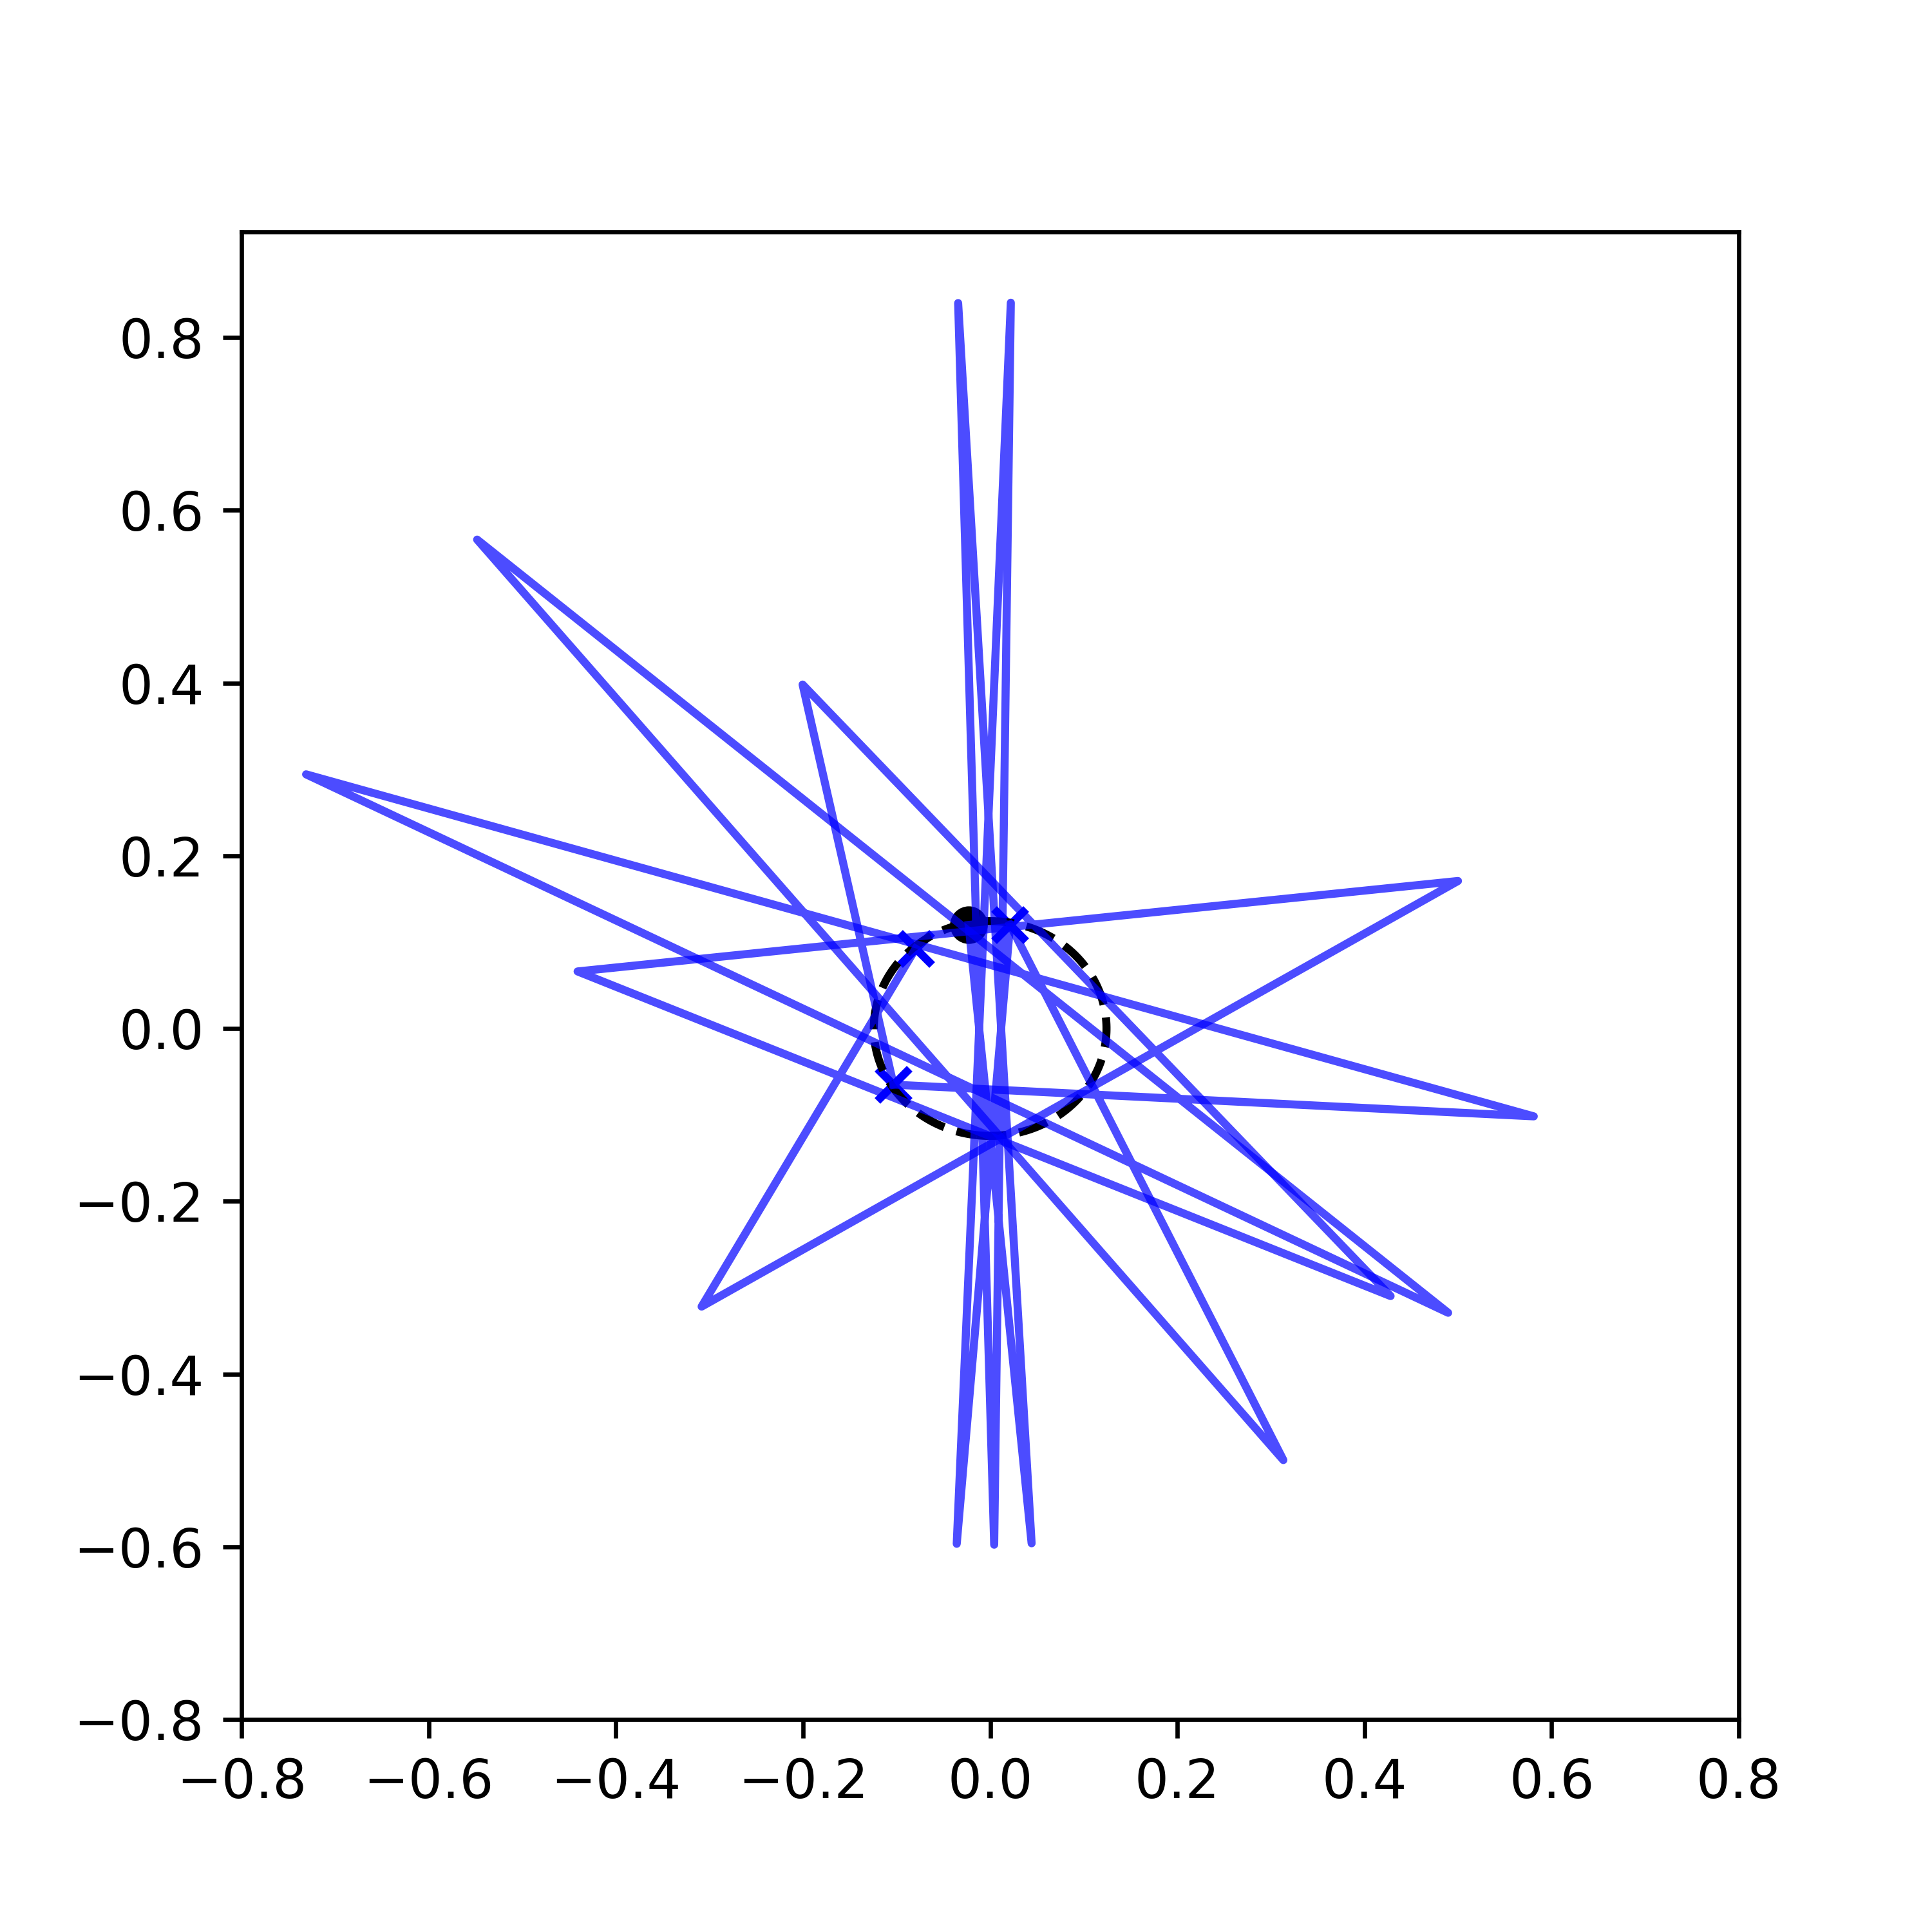
\includegraphics[scale=0.45]{figs/hmc_reflection_degenerate_example.png}
    \caption{Left: An iteration of HMC for LRPS with reflection and a chain of five samples on a standard-normal-likelihood-restricted uniform prior space.
    The black dot is the starting spot, each blue cross is a generated sample. Right: A later iteration of the same example. Note how every integration step contains a reflection and how far away the reflection points are from the actual boundary.}
    \label{fig:hmc_reflection_example}
\end{figure}

Having introduced Nested Sampling, we require one more piece of background knowledge before we are ready to tackle the contributions this thesis makes.
\FloatBarrier
\section{The Barrier Method}
This section provides an introduction to the Barrier Method, an algorithm for solving constrained convex optimization problems.
We will later incorporate ideas of this method into Nested Sampling.

The Barrier Method is used to solve optimization problems of the form
\begin{align}
    &\textrm{minimize} && f(x) && \nonumber\\
    &\textrm{subject to}  && f_i(x) \leq 0 \quad \textrm{for} \; i=1,...,m &&
    \label{eq:cvxproblem}
\end{align}
with $f$ and all $f_i$ being convex and twice continuously differentiable.
The problem also has to be strictly feasible, meaning that there exists an $\Tilde{x}$ in the domain of $f$, such that $f_i(\Tilde{x}) < 0 \; \forall i \in \{1,...,m\}$ \cite[561]{boyd}.

We reformulate the optimization problem from (\ref{eq:cvxproblem}) to be unconstrained by incorporating the constraints into the objective function.
\begin{align}
    &\textrm{minimize} && f(x) + \sum_{i=1}^m I(f_i(x))&& \label{eq:cvxproblem_unconstrained}
\end{align}
With $I(u)$ being defined as follows.
$$
I(u) = \begin{cases}
        0,      & \text{if }  u \leq 0\\
        \infty, & \text{if }  u > 0
        \end{cases}
$$
By applying an infinitely large penalty to infeasible points, (\ref{eq:cvxproblem_unconstrained}) accurately represents the original problem.
However, because the added terms are not differentiable, we would no longer be able to use gradient information to solve this formulation of the problem.
This is a problem because the most fundamental solver for optimization problems, Newton's Method, requires gradient information \cite[563]{boyd}.

To circumvent this shortcoming, we approximate $I$ using the log barrier function $\hat{I}(u)= -\frac{1}{t}\log(-u)$. $t$ is a parameter of the function, with larger $t$ leading to better approximations.
This behaviour can be seen in Figure \ref{fig:logbarrier}.
It should be noted that $\hat{I}$ is only defined for feasible points \cite[563]{boyd}.

\begin{figure}
    \centering
    \begin{tikzpicture}
    \begin{axis} [
        axis lines=center,
        xticklabel=\empty,
        yticklabel=\empty,
        xlabel=$u$,
        x label style={at={(axis description cs:0.5,-0.01)},anchor=north},
        ymax=1.8,
        xmax=0.4
    ]
    \addplot[
        domain=-2:0, 
        samples=100,
        color=blue,
        line width=0.1mm
    ] { 0 };
    \addplot[
        domain=-2:0, 
        samples=500,
        color=purple
    ] { -(1/1)*ln(-x) };
    \addplot[
        domain=-2:0, 
        samples=500,
        color=purple
    ] { -(1/4)*ln(-x) };
    \addplot[
        domain=-2:0, 
        samples=500,
        color=purple
    ] { -(1/16)*ln(-x) };
    \node[color=purple, anchor=west] at (axis cs: -0.7, 1.3) {t=1};
    \node[color=purple, anchor=west] at (axis cs: 0, 0.85) {t=4};
    \node[color=purple, anchor=west] at (axis cs: 0, 0.3) {t=16};
    \end{axis}
    \end{tikzpicture}
    \caption{Visualization of the exact barrier function $I$ in blue, and three log barrier functions (with $t=1,4,16$) in purple. The log barrier becomes a better approximation as $t$ increases.}
    \label{fig:logbarrier}
\end{figure}

The new, approximate optimization problem is:
\begin{align}
    &\textrm{minimize} && f(x) + \sum_{i=1}^m -\frac{1}{t}\log(-f_i(x))&&
    \label{eq:barrierproblem}
\end{align}
We can multiply the objective function by $t$ to obtain:
\begin{align}
    &\textrm{minimize} && t \cdot f(x) + \sum_{i=1}^m -\log(-f_i(x))&&
    \label{eq:objective}
\end{align}

By varying the parameter $t$, we obtain different problems with different solutions.
We will refer to the solution of (\ref{eq:objective}) for a certain value of $t$ as $x^*(t)$.
The set of solutions for all possible values of $t$, $\{x^*(t) \,|\, t > 0\}$, is called the central path of the problem.
It converges to the true solution as $t \rightarrow \infty$, as can be seen in Figure \ref{fig:barrier_method_example} \cite[564]{boyd}.

\begin{figure}
    \centering
    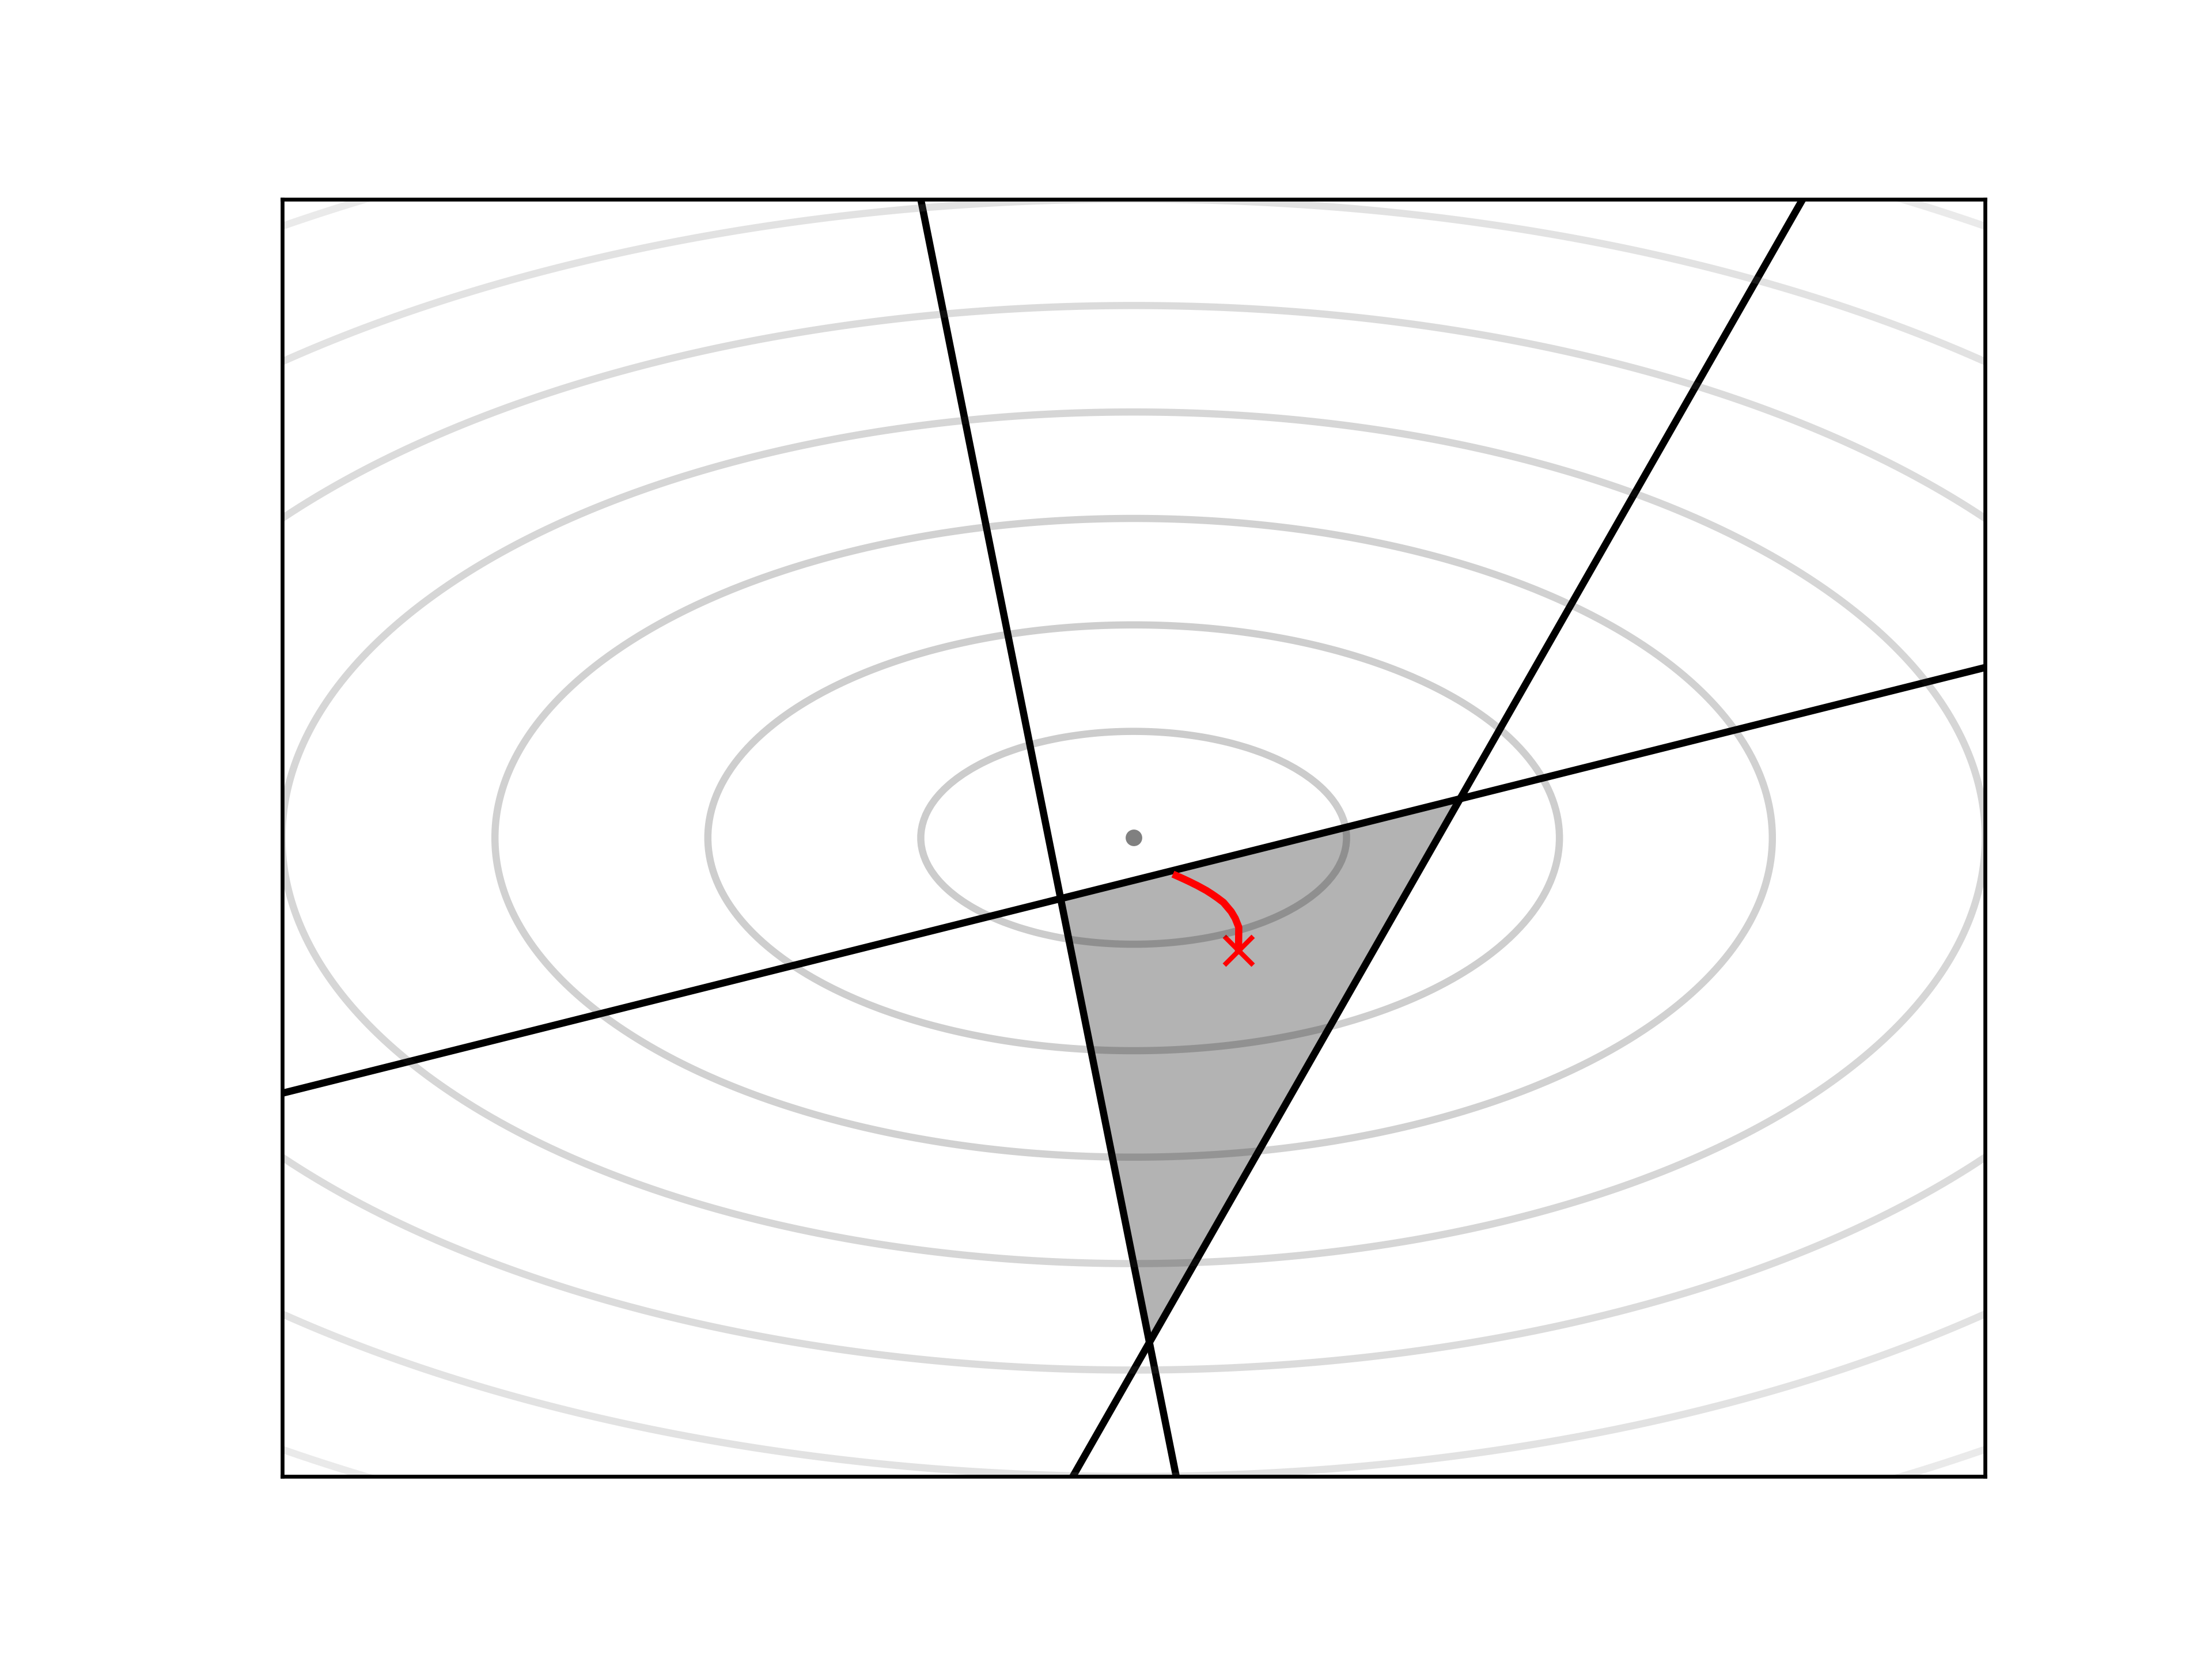
\includegraphics[scale=0.6]{figs/barrier_method_example.png}
    \caption{Central path of an example optimization problem. The shaded area is the feasible region, given by the constraint functions in black. The grey lines indicate contours of the objective function, with the unconstrained optimum at the grey dot. The central path of the problem is shown in red. $x^*(1)$ is marked by a red cross.}
    \label{fig:barrier_method_example}
\end{figure}

Solving the problem in (\ref{eq:objective}) for a large value of $t$ provides a good estimation of the exact solution.
$x^*(t)$ is provably $\frac{m}{t}$-suboptimal, meaning that its objective function value is at most $\frac{m}{t}$ greater than the optimal value \cite[566]{boyd}.

However, as the log barrier function becomes a better approximation of the strict barrier with larger $t$, its derivatives become more extreme.
This causes the standard optimization procedures, such as Newton's method, to fail \cite[564]{boyd}.
The Barrier Method is an approach that solves this issue by applying an iterative strategy.
In each iteration, $x^*(t_i)$ is computed using Newton's Method (called a centering step).
The value of $t_i$ increases with each iteration, and the result of the last iteration is used as the starting point for the current one.
This stabilizes the centering steps \cite[569]{boyd}. 

\begin{algorithm}
    \caption[The basic Barrier Method.]{BarrierMethod ($x_0$, $t_0$, $\mu$, $\epsilon$)}
    \label{alg:product_axes}
    \begin{algorithmic}
        \State $x \gets x_0$
        \State $t \gets t_0$
        \Repeat
            \State compute $x^*(t)$ by minimizing $t \cdot f(x) + \sum_{i=1}^m -\log(-f_i(x))$ starting at $x$
            \State $x \gets x^*(t)$
            \State $\hat{\epsilon} \gets \frac{m}{t}$
            \State $t \gets \mu t$
        \Until{$\hat{\epsilon} < \epsilon$}
        \State return $x$
    \end{algorithmic}
\end{algorithm}

The most important idea we borrow from the Barrier Method is how the log barrier function provides a way to make a hard boundary soft and differentiable.
In the next chapter, we incorporate this idea into the LRPS step of Nested Sampling.


\chapter{Nested Sampling with Barriers}

\section{Motivation}
As was shown in Section 1.4, LRPS is difficult.
Because the likelihood-constraint grows tighter and the ratio of valid area to the area of the whole sample space decreases steadily, finding samples within the constraint boundary becomes more difficult with every Nested Sampling iteration.
For methods like Rejection Sampling and the Metropolis algorithm, this manifests in low acceptance rates of proposals, which lead to wasted computational work.
For HMC adapted to LRPS, detecting the point at which the particle breaches the likelihood-constraint-boundary and must be reflected also becomes harder, since the distance the particle can travel before leaving the valid region decreases with each iteration.
All these methods only notice the likelihood constraint boundary once they have crossed it.
The proposals for Rejection Sampling and the Metropolis Algorithm do not take into account the likelihood at all, having to reject (intermediate) samples that cross the boundary, and while HMC for LRPS can reflect during proposal generation, this only happens after the boundary has been crossed.
We would like an approach that softens the hard likelihood constraint and pushes the samples away from the boundary during sampling.

Thinking back to the Barrier Method, we can make the following observation:
The log barrier also softens a hard constraint function and allows the optimization algorithm to feel the constraint before crossing it.
This leads us to the main idea of this thesis: incorporating the log barrier from the Barrier Method into the LRPS step of Nested Sampling.

\section{Derivation}
\subsection{Deriving the log barrier term}
In this section we draw parallels between LRPS and convex optimization to find a way to use log barriers in a probabilistic setting.

In convex optimization, we minimize a function constrained by a set of convex functions (as can be seen in (\ref{eq:cvxproblem})).
In LRPS, we sample from a probability distribution $\pi(\theta)$, constrained by $L(\theta) > L^*$.
Even though this constraint is not necessarily convex (for most real-world applications it will not be), it still takes on a similar role to the constraint functions in convex optimization.
By viewing LRPS through the lens of optimization, we are able to apply the ideas of Chapter 2 to it.
That said, we are only doing this for inspiration.
We will not be solving the optimization problem we set up.
\begin{align}
    &\textrm{maximize} \quad \pi(\theta) &&\textrm{subject to} \quad L(\theta) > L^* \nonumber\\
    \iff &\textrm{minimize} \quad -\log(\pi(\theta)) &&\textrm{subject to} \quad L(\theta) > L^* \nonumber\\
    \iff &\textrm{minimize} \quad -\log(\pi(\theta)) &&\textrm{subject to} \quad l^* - l(\theta) < 0 \label{eq:log_barrier_derivation_1}\\
    \iff &\textrm{minimize} \quad -\log(\pi(\theta)) + I(l^* - l(\theta)) \nonumber
\end{align}
Optimization problems over probabilities are usually solved in logarithmic space rather than probability space for reasons like easier differentiation and numerical stability.
We do the same, taking the logarithm of both the objective function and both sides of the likelihood constraint.
Note that $l(\theta) = \log(L(\theta))$ and $l^* = \log(L^*)$ in (\ref{eq:log_barrier_derivation_1}).
Next, we generate the associated approximate problem using log barriers (see (\ref{eq:barrierproblem})).
\begin{align*}
    &\textrm{minimize} \quad -\log(\pi(\theta)) + \hat{I}(l^* - l(\theta)) \\
    \iff &\textrm{minimize} \quad -\log(\pi(\theta)) - \frac{1}{t}\log(l(\theta) - l^*)
\end{align*}
By moving the resulting objective function back into probability space, we obtain a term that will be important for the rest of this thesis.
\begin{align}
    &\exp(-(-\log(\pi(\theta)) - \frac{1}{t}\log(l(\theta) - l^*))) \nonumber\\
    = \, &\pi(\theta) \, (l(\theta) - l^*)^{\frac{1}{t}} \label{eq:log_barrier_term}
\end{align}
We call $(l(\theta) - l^*)^\frac{1}{t}$ the log barrier term.
For valid $\theta$, as the (log-)likelihood of $\theta$ approaches the minimum (log-)likelihood, the log barrier term decreases, making values of $\theta$ close to the likelihood-restriction boundary less likely.
In the next section we integrate this term into Nested Sampling.

\subsection{Incorporating the log barrier term}
Having derived a way to represent log barriers for probabilities, we are now looking for a way to use them during LRPS without introducing a bias into our sampler.

To this end, we expand the sampling space by adding a one-dimensional real variable $q$, taking values in $(q_{\textrm{min}}, q_{\textrm{max}})$.
$$
\theta \rightarrow (\theta, q)
$$
We define $q$ to be independent of $\theta$.
$$
P(\theta, q) = P(\theta) \; P(q)
$$
By considering Bayes' rule (see (\ref{eq:bayes})), we can see that the independence follows through to the likelihood:
\begin{align*}
    P(\theta, q | D) &= P(\theta | D) \; P(q | D) \\
    &= \frac{P(D | \theta) \; P(\theta)}{\int_\Theta P(D | \theta) \; P(\theta) \; d\theta} \; \frac{P(D | q) \; P(q)}{\int_Q P(D | q) \; P(q) \; dq} \\
    &= \frac{P(D | \theta) \; P(\theta) \; P(D | q) \; P(q)}{\int_\Theta P(D | \theta) \; P(\theta) \; d\theta \; \int_Q P(D | q) \; P(q) \; dq} \\
    &= \frac{P(D | \theta) \; P(D | q) \;\; P(\theta) \; P(q)}{\int_\Theta P(D | \theta) \; P(\theta) \; d\theta \; \int_Q P(D | q) \; P(q) \; dq} \\
    &= \frac{L(\theta) \; L(q) \;\; \pi(\theta) \; \pi(q)}{Z_\theta \; Z_q} \\
    &= \frac{L(\theta, q) \; \pi(\theta, q)}{Z_{\theta, q}}
\end{align*}
This lets us freely choose the likelihood and prior of our new variable $q$.
It also shows that we can perform Nested Sampling on the $(\theta, q)$-space and recover the original evidence $Z_\theta$ by dividing $Z_{\theta, q}$ by $Z_q$.

Now, let us take a look at LRPS on this expanded space.
We will call the likelihood-restricted prior $\bar{\pi}$.
\begin{align*}
    (\theta,q) \sim \; &\bar{\pi}(\theta, q \,|\, L^*) \\
    &\bar{\pi}(\theta, q \,|\, L^*) = \pi(\theta, q) \, \mathbbm{1}_{\{L(\theta, q) \, > \, L^*\}}
\end{align*}
$\mathbbm{1}_{\{f(x)\}}$ with a predicate $f$ is short for the indicator function $\mathbbm{1}_{\{x \,|\, f(x)\}}(x)$ and is $1$ whenever the predicate is fulfilled and $0$ otherwise.

We employ a technique called collapsed Gibbs sampling \cite{collapsed_gibbs} to sample from the likelihood-restricted prior.
By first sampling from the marginal distribution of $\theta$, we can then use the obtained value to sample from the conditional distribution of $q$.
\begin{align*}
    \theta &\sim  \bar{\pi}(\theta \,|\, L^*) \\
    q &\sim  \bar{\pi}(q \,|\, L^*, \theta)
\end{align*}
By defining the likelihood of $q$ as $L(q) = \frac{1}{q}$, we can reshape the likelihood-restricted priors:
\begin{align*}
    \bar{\pi}(\theta \,|\, L^*) &= \int_{q_{\textrm{min}}}^{q_{\textrm{max}}} \bar{\pi}(\theta, q \,|\, L^*) \; dq \\
    &= \int_{q_{\textrm{min}}}^{q_{\textrm{max}}} \pi(\theta) \, \pi(q) \, \mathbbm{1}_{\{L(\theta, q) \,>\, L^*\}} \; dq \\
    &= \pi(\theta) \int_{q_{\textrm{min}}}^{q_{\textrm{max}}} \pi(q) \, \mathbbm{1}_{\{L(\theta) \, L(q) \,>\, L^*\}} \; dq \\
    &= \pi(\theta) \int_{q_{\textrm{min}}}^{q_{\textrm{max}}} \pi(q) \, \mathbbm{1}_{\{L(\theta) / q \,>\, L^*\}} \; dq \\
    &= \pi(\theta) \int_{q_{\textrm{min}}}^{q_{\textrm{max}}} \pi(q) \, \mathbbm{1}_{\{q \,<\, L(\theta) / L^*\}} \; dq \\
    &= \pi(\theta) \int_{q_{\textrm{min}}}^{L^* / L(\theta)} \pi(q) \; dq \\
    &= \pi(\theta) \; \Pi_q(L(\theta) / L^*) \\
    \bar{\pi}(q \,|\, L^*, \theta) &= \pi(q) \, \mathbbm{1}_{\{q < L(\theta) / L^*\}}
\end{align*}
Where $\Pi_q$ is the CDF of $q$.
Since we are free to define $\Pi_q$ however we want, we can use it to insert the log barrier term from (\ref{eq:log_barrier_term}).
\begin{align*}
    \Pi_q(L(\theta) / L^*) &\overset{!}{=} (l(\theta) - l^*)^{\frac{1}{t}} \\
    \Pi_q(L(\theta) / L^*) &=(\log(L(\theta)) - \log(L^*))^{\frac{1}{t}} \\
    \Pi_q(L(\theta) / L^*) &= \log(L(\theta) / L^*)^{\frac{1}{t}} \\
    \textrm{let } q &= L(\theta) / L^* \\
    \Pi_q(q) &= \log(q)^{\frac{1}{t}}
\end{align*}
With this, we have defined the shape of the CDF of $q$ in such a way that the log barrier term appears in LRPS.
However, as can be seen in Figure \ref{fig:unnormalized}, the CDF of $q$ is unnormalized unless we choose $q_{\textrm{max}}=e$.

\begin{figure}
    \centering
    \begin{tikzpicture}
    \begin{axis} [
        axis lines=center,
        xlabel=$q$,
        x label style={at={(axis description cs:0.5,-0.1)},anchor=north},
        xmin=0,
        xmax=5,
        ymax=2
    ]
    \addplot[
        domain=1:10, 
        samples=500,
        color=red
    ] { ln(x)^(1/0.5) };
    \addplot[
        domain=1:10, 
        samples=500,
        color=blue
    ] { ln(x)^(1/1) };
    \addplot[
        domain=1:10, 
        samples=500,
        color=green
    ] { ln(x)^(1/4) };
    \node[color=red, anchor=east] at (axis cs: 3.8, 1.9) {t=0.5};
    \node[color=blue, anchor=east] at (axis cs: 4.7, 1.6) {t=1};
    \node[color=green, anchor=east] at (axis cs: 4.5, 1.0) {t=4};
    \end{axis}
    \end{tikzpicture}
    \caption{Visualization of the unnormalized CDF $\Pi_q$ of $q$ for different values of $t$ and $q_{\textrm{max}}=5$.}
    \label{fig:unnormalized}
\end{figure}

We can normalize it for any other $q_{\textrm{max}}$ by scaling $\Pi_q$ to have a value of $1$ at $q=q_{\textrm{max}}$.
We called the normalized version $\hat{\Pi}_q$.
$$
\hat{\Pi}_q(q) = \frac{\Pi_q(q)}{\Pi_q(q_{\textrm{max}})} \quad \textrm{if } q \in (1, q_{\textrm{max}})
$$
Note that there is no need to shift $\hat{\Pi}_q$ to have value $0$ at a different $q_{\textrm{min}}$ than $1$.
$q_{\textrm{min}}=1$ is a natural choice as $\hat{\Pi}_q(L(\theta) - L^*)$ should be $0$ for $L(\theta) - L^* < 1$, because then the likelihood-constraint is not satisfied.
In all, we define the CDF for $q$ as follows:
$$
\hat{\Pi}_q(q) = 
\begin{cases}
    0 & \text{if } q \leq 1 \\
    \frac{\log(q)^\frac{1}{t}}{\log(q_{\textrm{max}})^\frac{1}{t}} & \text{if } q \in (1, q_{\textrm{max}})\\
    1 & \text{if } q \geq q_{\textrm{max}}
\end{cases}
$$

Differentiating $\hat{\Pi}_q$ gives us the PDF of $q$.
$$
    \frac{\textrm{d} \, \Pi_q}{\textrm{d} \, q} (q) = \pi(q) = 
    \begin{cases}
        0 & \text{if } q \leq 1 \\
        \frac{\log(q)^{\frac{1}{t}-1}}{tq\log(q_{\textrm{max}})^\frac{1}{t}} & \text{if } q \in (1, q_{\textrm{max}})\\
        0 & \text{if } q \geq q_{\textrm{max}}
    \end{cases}
$$

With that, we have defined both the likelihood and the prior of $q$ in a way that incorporates the log barrier term into LRPS.
This lets us write down the modified version of Nested Sampling in Algorithm \ref{alg:barriersampling}.
The changes from the original are the following:
\begin{enumerate}
    \item For each starting $\theta$, also sample a $q$.
    \item Use the joint likelihoods of $\theta$ and $q$, $L(\theta, q) = \frac{L(\theta)}{q}$, instead of just the likelihood of $\theta$.
    \item Sample new $\theta$ from the modified constrained prior $\pi_\theta(\theta) \, \Pi_q(l(\theta) - l^*)$.
    \item Sample new $q$ from the constrained prior $\pi_q(q) \, \mathbbm{1}_{\{q < L(\theta_{\textrm{new}}) / L^*\}}$ dependent on the sampled $\theta$.
    \item Divide out $Z_q(t, q_{\textrm{max}})$ from the evidence before returning it.
\end{enumerate}
\vspace{0.25cm}

The $q$-evidence $Z_q$ is a function of $t$ and $q_{\textrm{max}}$, and can be computed analytically:
\begin{align}
    Z_q(t, q_{\textrm{max}}) &= \int_1^{q_{\textrm{max}}} L(q) \, \pi(q) \, dq \nonumber\\
    &= \int_1^{q_{\textrm{max}}} \frac{\log(q)^{\frac{1}{t}-1}}{tq^2\log(q_{\textrm{max}})^\frac{1}{t}} \, dq \nonumber\\
    &= \frac{1}{t \log(q_{\textrm{max}})^{\frac{1}{t}}} \int_1^{q_{\textrm{max}}} \frac{\log(q)^{\frac{1}{t}-1}}{q^2} \, dq \nonumber\\
    &\mathrel{\overset{\makebox[0pt]{\mbox{\normalfont\tiny int. by sub.}}}{=}} \quad \frac{1}{t \log(q_{\textrm{max}})^{\frac{1}{t}}} \int_0^{\log(q_{\textrm{max}})} u^{\frac{1}{t}-1} e^{-u} \, du \label{eq:sub_zq_1}
\end{align}
The substitution used is $u = \log(q)$.
Now we use the definition of the lower incomplete gamma function:
\begin{align}
    \Gamma(a, x) &= \int_x^{\infty} u^{a-1} e^{-u} \, du \nonumber\\
    \Gamma(a, x) - \Gamma(a, y) &= \int_x^{\infty} u^{a-1} e^{-u} \, du - \int_y^{\infty} u^{a-1} e^{-u} \, du \nonumber\\
    \textrm{for } y > x\textrm{:} \quad \Gamma(a, x) - \Gamma(a, y) &= \int_x^y u^{a-1} e^{-u} \, du \label{eq:gamma_diff}
\end{align}
By setting $a = \frac{1}{t}$, $x = 0$ and $y = \log(q_{\textrm{max}})$, we can apply (\ref{eq:gamma_diff}) to (\ref{eq:sub_zq_1}):
\begin{align*}
    Z(t, q_{\textrm{max}}) &= \frac{1}{t \log(q_{\textrm{max}})^{\frac{1}{t}}} \int_0^{\log(q_{\textrm{max}})} u^{\frac{1}{t}-1} e^{-u} \, du \\
    &= \frac{\Gamma(\frac{1}{t}, 0) - \Gamma(\frac{1}{t}, \log(q_{\textrm{max}}))}{t \log(q_{\textrm{max}})^{\frac{1}{t}}}
\end{align*}

\begin{algorithm}
    \caption[Nested Sampling with the log barrier term.]{NestedBarrierSampling ($n$, $\epsilon$, $\pi_\theta$, $L_\theta$, $t$, $q_{\textrm{max}}$)}
    \label{alg:barriersampling}
    \begin{algorithmic}
        \State sample $\theta_1 ... \theta_n$ from the prior $\pi_\theta$
        \State sample $q_1 ... q_n$ from the prior $\pi_q$
        \State $live\_points \gets [ (\theta_1, q_1) ... (\theta_n, q_n) ]$
        \State $mass \gets 1$
        \State $dead\_points \gets [ \; ]$
        \State $Z \gets 0$
        \Repeat
            \State $L_{\textrm{min}} \gets \min_{(\theta,q) \, \in \, live\_points} L(\theta, q)$ 
            \State $(\theta_{\textrm{min}}, q_{\textrm{min}}) \gets \textrm{argmin}_{(\theta,q) \, \in \, live\_points} L(\theta, q)$ 
            \State remove $(\theta_{\textrm{min}}, q_{\textrm{min}})$ from $live\_points$
            \State append $\theta_{\textrm{min}}$ to $dead\_points$
            \State sample $f$ from  $\textrm{Beta}(1, n)$
            \State $mass\_shell \gets mass \cdot f$
            \State $mass \gets mass - mass\_shell$
            \State $Z \gets Z + mass\_shell \cdot L_{\textrm{min}}$
            \State sample $\theta_{\textrm{new}}$ from $\hat{\pi}_\theta(\theta) \, \Pi_q(l(\theta) - l^*)$
            \State sample $q_{\textrm{new}}$ from $\pi_q(q) \, \mathbbm{1}_{\{q \,<\, L(\theta_{\textrm{new}}) / L^*\}}$
            \State append $(\theta_{\textrm{new}}, q_{\textrm{new}})$ to $live\_points$
            \State $L_{\textrm{max}} \gets \max_{(\theta,q) \, \in \, live\_points} L(\theta, q)$ 
        \Until{$(mass \cdot L_{\textrm{max}}) / Z < \epsilon$}
        \State $Z_\theta \gets Z / Z_q(t, q_{\textrm{max}})$
        \State return $Z_\theta,\, dead\_points$
    \end{algorithmic}
\end{algorithm}

With that, we have successfully defined a version of Nested Sampling that incorporates the log barrier term from (\ref{eq:log_barrier_term}).
Next, we will examine the newly introduced parts of the algorithm, namely the auxiliary variable $q$ and the parameters $t$ and $q_{\textrm{max}}$.

\FloatBarrier
\section{Interpretation}
In this section, we analyse the elements of Nested Sampling with Barriers we introduced in the previous section.

\subsection{Interpreting $q$}
Each sample from the original $\theta$-space gets an auxiliary $q$ in Nested Sampling with Barriers.
Because $L(\theta, q) = \frac{L(\theta)}{q}$ and $q > 1$, the likelihood of each $\theta$ is reduced by its $q$.
Since $Z_q$ is divided out later, this does not influence the final evidence and is only relevant for the likelihood-threshold each point generates when it is removed from the live points.
The larger the $q$, the more the likelihood is reduced.
Since $q$ is sampled from $\pi_q(q) \, \mathbbm{1}_{\{q < L(\theta_{\textrm{new}}) / L^*\}}$, the $\theta$ that are further away from the likelihood-constraint are expected to have higher $q$ values, reducing their likelihood more.
This can be interpreted as making up for the fact that the log barrier term discourages sampling close to the likelihood-constraint.
If the likelihoods were kept the same, the likelihood-constraint would increase much more quickly.

\subsection{Influence of $t$ and $q_{\textrm{max}}$}
$t$ and $q_{\textrm{max}}$ determine the shape and support of the distribution of $q$.
Since the log barrier term is incorporated using the CDF of $q$, they also influence how the log barrier term acts.

\begin{figure}
    \begin{minipage}{0.45\textwidth}
        \begin{tikzpicture}
            \begin{axis} [
                axis lines=center,
                xlabel=$q$,
                x label style={at={(axis description cs:0.5,-0.1)},anchor=north},
                xmax=2,
                scale=0.85
            ]
            \addplot[
                domain=1:2, 
                samples=1000,
                color=red
            ] { ln(x)^(1/0.5 - 1) / (0.5*x*ln(2)^(1/0.5)) };
            \addplot[
                domain=1:2, 
                samples=500,
                color=blue
            ] { ln(x)^(1/1 - 1) / (1*x*ln(2)^(1/1)) };
            \addplot[
                domain=1:2, 
                samples=500,
                color=green
            ] { ln(x)^(1/2 - 1) / (2*x*ln(2)^(1/2)) };
            \node[color=red, anchor=west] at (axis cs: 1.8, 2.1) {t=0.5};
            \node[color=blue, anchor=west] at (axis cs: 1.25, 2.0) {t=1};
            \node[color=green, anchor=west] at (axis cs: 1.03, 4) {t=2};
            \end{axis}
            \end{tikzpicture}
    \end{minipage}
    \begin{minipage}{0.45\textwidth}
        \begin{tikzpicture}
            \begin{axis} [
                axis lines=center,
                xlabel=$q$,
                x label style={at={(axis description cs:0.5,-0.1)},anchor=north},
                xmax=2,
                scale=0.85
            ]
            \addplot[
                domain=1:2, 
                samples=1000,
                color=red
            ] { ln(x)^(1/0.5) / (ln(2)^(1/0.5)) };
            \addplot[
                domain=1:2, 
                samples=500,
                color=blue
            ] { ln(x)^(1/1) / (ln(2)^(1/1)) };
            \addplot[
                domain=1:2, 
                samples=500,
                color=green
            ] { ln(x)^(1/2) / (ln(2)^(1/2)) };
            \node[color=red, anchor=west] at (axis cs: 1.6, 0.4) {t=0.5};
            \node[color=blue, anchor=west] at (axis cs: 1.35, 0.4) {t=1};
            \node[color=green, anchor=west] at (axis cs: 1.18, 0.7) {t=2};
            \end{axis}
            \end{tikzpicture}
    \end{minipage}
    \caption{Visualization of the normalized PDF (left) and normalized CDF (right) of $q$ for different values of $t$ and $q_{\textrm{max}}=2$.}
    \label{fig:q_normalized}
\end{figure}

A larger value for $q_{\textrm{max}}$ lets the log barrier term affect sampling earlier (for $\theta$ further away from the likelihood-constraint-boundary); a smaller $q_{\textrm{max}}$ confines the influence of the barrier term to a smaller region close to the likelihood-constraint-boundary.
As discussed in Section 1.5, $t$ determines how closely the log barrier approximates the true barrier.
A large $t$ leads to a better approximation, generating a steeper barrier, and making the log barrier term act less strongly in regions further away from the likelihood-constraint-boundary (see Figure \ref{fig:q_normalized}).
Lower values of $t$ give the log barrier term more influence even in these regions.
We will see how $t$ and $q_{\textrm{max}}$ practically influence the algorithm's performance in Section 2.5.

In the next section, we discuss, in theory, which methods for LRPS can make use of the introduced log barrier term.

\section{Implementation of LRPS}
As with the standard Nested Sampling algorithm, the step of likelihood-restricted prior sampling in the original $\theta$-space still exists (see line 16 of Algorithm \ref{alg:barriersampling}).
However, we now have the log barrier term affecting the sampling, which we can make use of.
In this section we recapitulate the options for LRPS presented in Section 1.4 and describe how they may benefit from the log barrier term introduced by Nested Sampling with Barriers.

\subsection{Rejection Sampling and Discretized LRPS}
Because they are not MCMC methods, these techniques do not benefit from the log barrier term.
Rejection sampling proposals are not affected by the log barrier term, so their acceptance rates stay the same as with standard Nested Sampling.
Discretized LRPS has no problem with acceptance rates, only with how many discrete points are needed for high-dimensional spaces, which Nested Sampling with Barriers does not help with.

\subsection{Metropolis Algorithm}
The Metropolis algorithm for LRPS can make use of the log barrier term.
When a Metropolis Markov chain gets close to the likelihood-constraint-boundary, the log barrier term discourages it from sampling even closer.
If the step size is chosen small enough, this may drastically reduce the number of invalid proposals (proposals violating the likelihood-constraint).
To ensure efficient exploration of the $\theta$-space for the whole Nested Sampling procedure, during which the explorable space continually shrinks, an adaptive step size is still required.

\subsection{Hamiltonian Monte Carlo}
Like the Metropolis algorithm, HMC benefits from the log barrier term.
It does so especially, since the log barrier term curves the negative log density surface, on which the HMC particles move, upwards as it gets closer to the likelihood-constraint-boundary.
This causes the particles to turn away before they hit the boundary (see Figure \ref{fig:barrier_sampling_hmc}), and leads to all proposals being valid.
This way, the particles do not have to be reflected off the boundary.
An adaptive step size is still worth implementing with this method, since the later iterations of Nested Sampling have such tiny valid spaces that the boundary may otherwise be crossed before it can be felt.

\begin{figure}
    \centering
    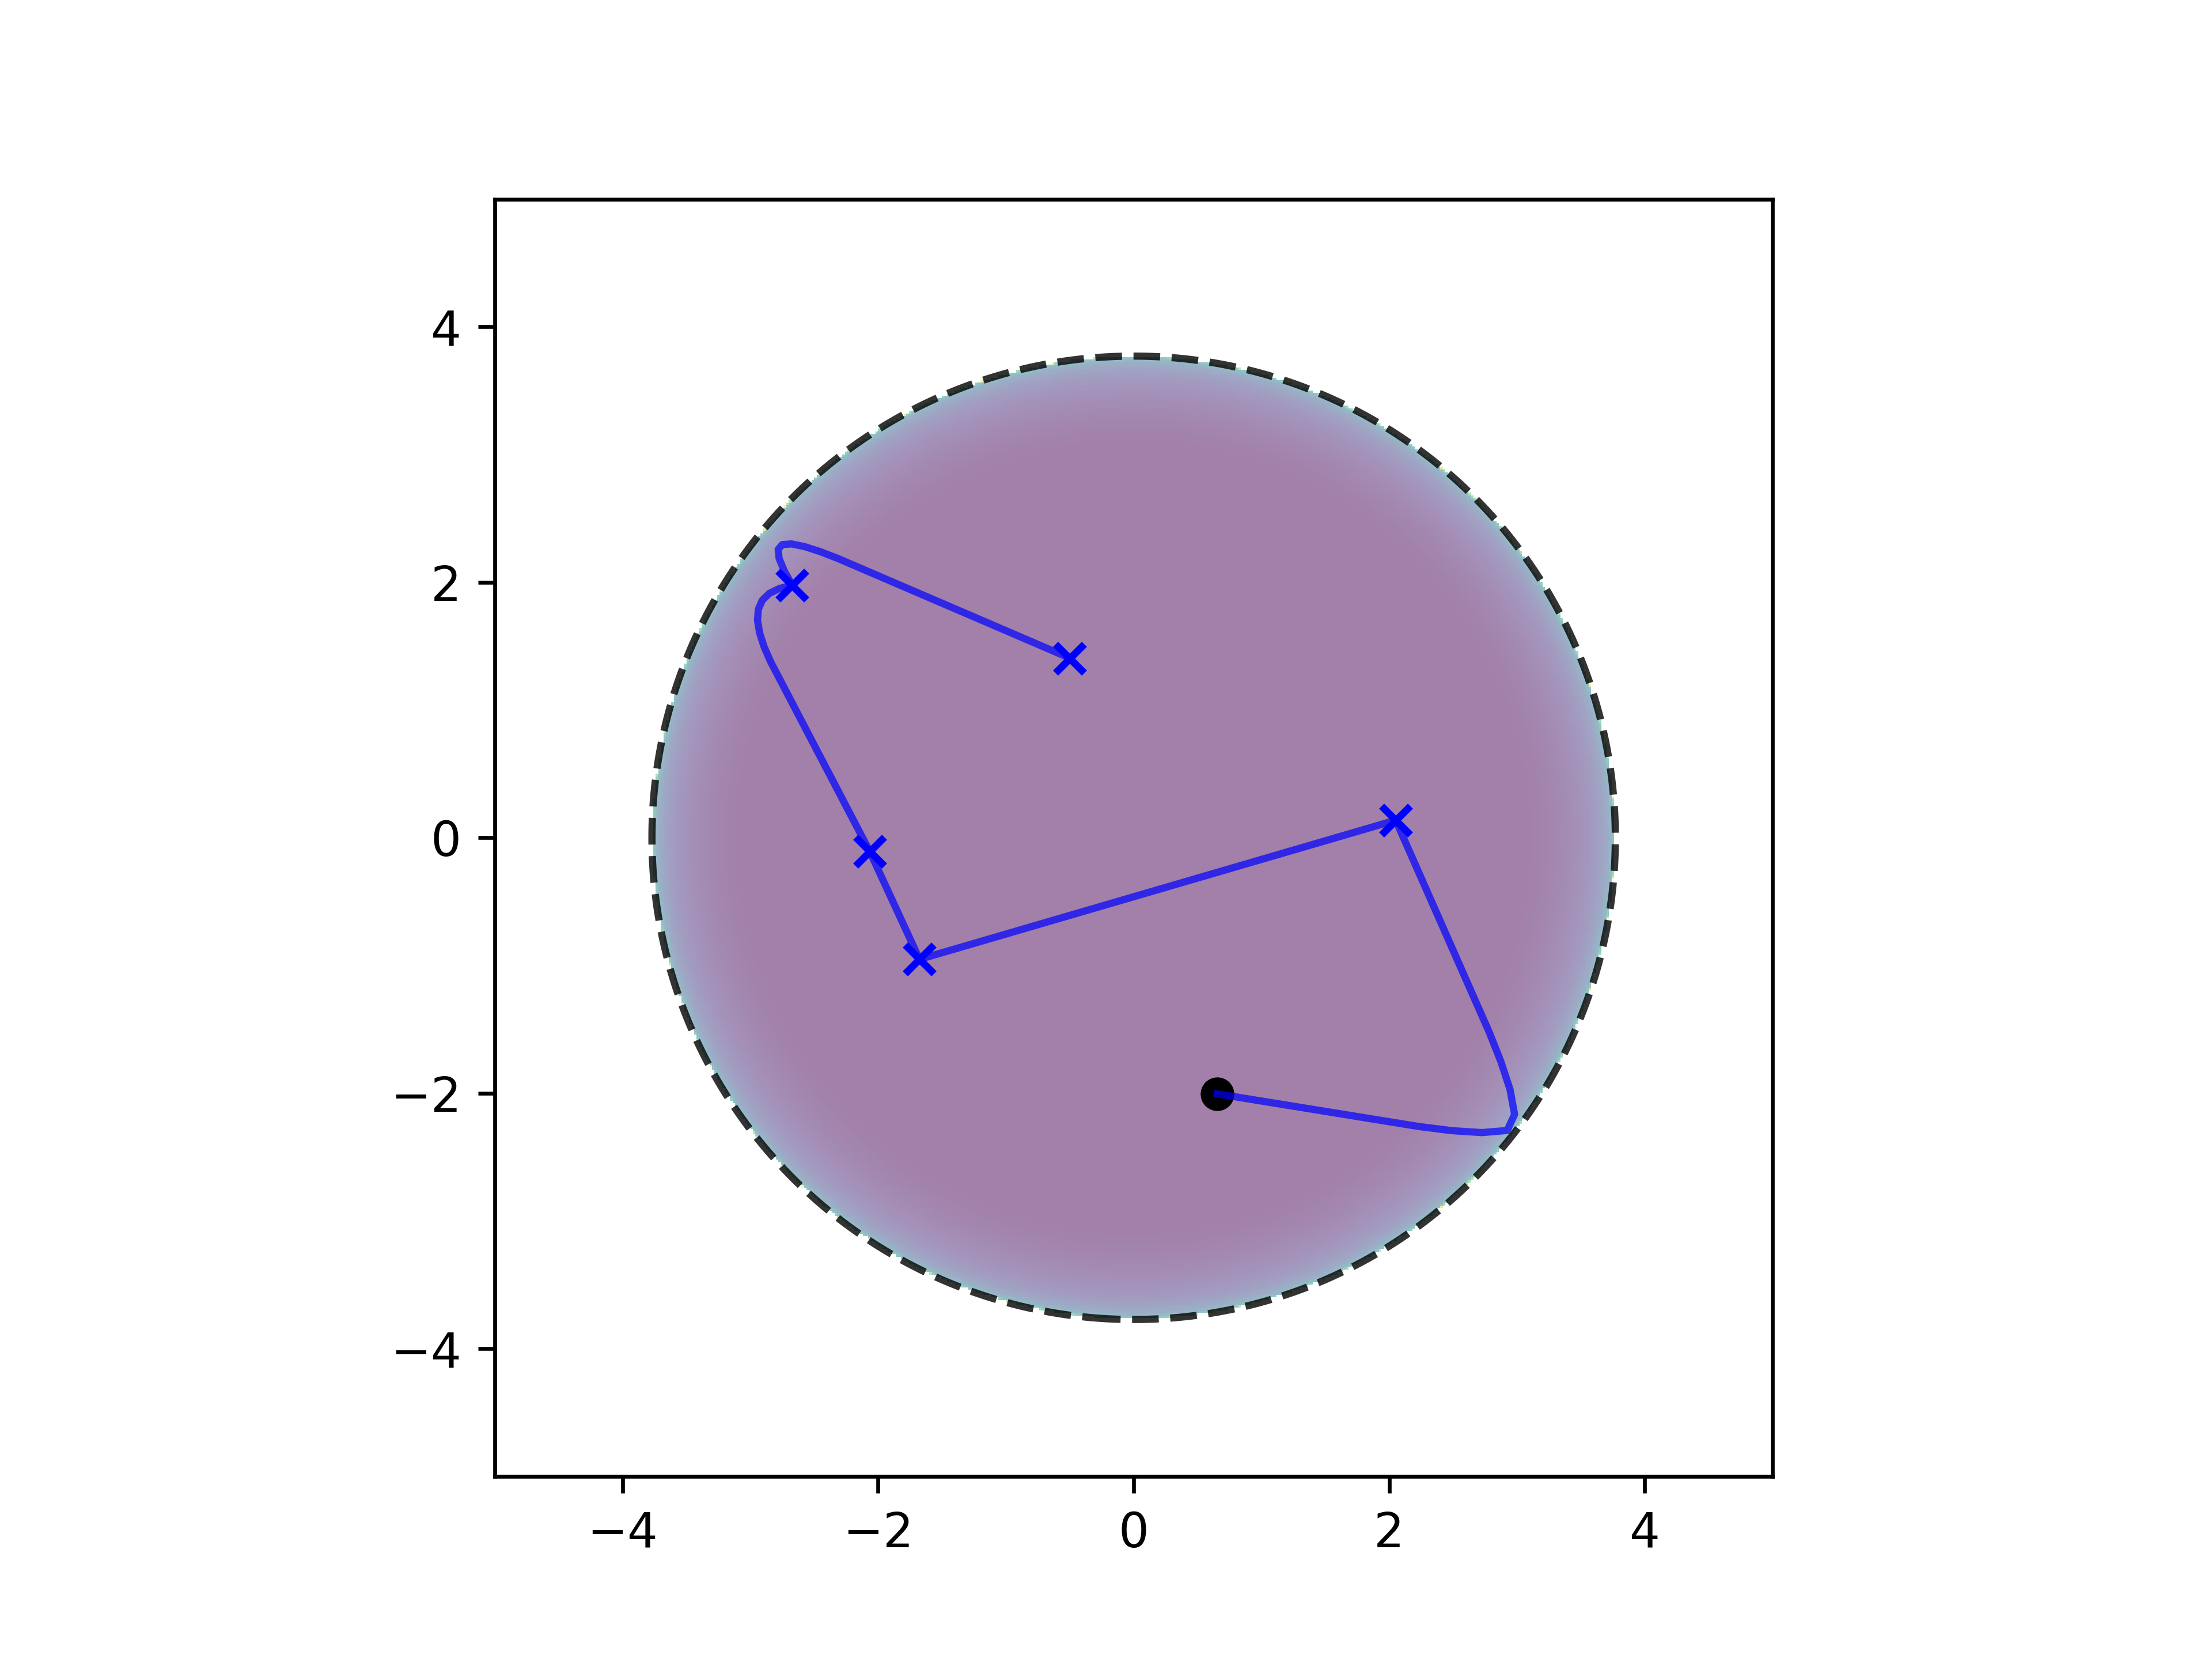
\includegraphics[scale=0.8]{figs/barrier_sampling_hmc.png}
    \caption{A run of HMC for LRPS with a chain of five samples on a standard-normal-likelihood-restricted uniform prior space.
    The black dot is the starting spot, each blue cross is a generated sample.
    The background color shows the negative log density the particles move on, with lighter colors representing higher values.}
    \label{fig:barrier_sampling_hmc}
\end{figure}



\FloatBarrier
\section{Results}
This chapter contains the results of a number of experiments on Nested Sampling with Barriers.
First, I show how Nested Sampling with Barriers compares to standard Nested Sampling using multiple example problems.
I then demonstrate the influence of the parameters $t$ and $q_{\textrm{max}}$ on Nested Sampling with Barriers on one example problem.

\subsection{Nested Sampling with and without Barriers}
Both standard Nested Sampling and the Barriers variant were tested on four example problems with the following likelihood functions:
\begin{itemize}
    \item a 2D slab and spike
    \item a 20D slab and spike
    \item a 2D mixture of 5 nonconcentric Gaussians
    \item a 20D mixture of 5 nonconcentric Gaussians 
\end{itemize}
The slab-and-spike problems are taken from Skilling's introductory paper on Nested Sampling \cite{skilling}, where it serves as an example of a type of problem Nested Sampling is well-suited for.
The nonconcentric Gaussians are example problems with multimodality, which remains difficult for MCMC methods to do well with.
The examples' likelihoods are defined in the following piece of Python code:
\vspace{0.4cm}

\hrule
\begin{lstlisting}[language=Python]
def spike_likelihood(x, dim):
    slab = 100 * multivariate_normal.pdf(x, mean=np.zeros(dim), cov=np.eye(dim)*0.01)
    spike = multivariate_normal.pdf(x, mean=np.zeros(dim), cov=np.eye(dim)*0.1)
    return slab + spike

gauss_2d_mus = [np.array([-2,-2]), np.array([-2,2]), np.array([0,0]), np.array([2,-2]), np.array([2, 2])]
gauss_20d_mus = [np.array([-2,-2,-2,-2,-2,-2,-2,-2,-2,-2,-2,-2,-2,-2,-2,-2,-2,-2,-2,-2]),
                 np.array([ 2, 2, 2, 2, 2, 2, 2, 2, 2, 2,-2,-2,-2,-2,-2,-2,-2,-2,-2,-2]),
                 np.array([ 0, 0, 0, 0, 0, 0, 0, 0, 0, 0, 0, 0, 0, 0, 0, 0, 0, 0, 0, 0]),
                 np.array([-2,-2,-2,-2,-2,-2,-2,-2,-2,-2, 2, 2, 2, 2, 2, 2, 2, 2, 2, 2]),
                 np.array([ 2, 2, 2, 2, 2, 2, 2, 2, 2, 2, 2, 2, 2, 2, 2, 2, 2, 2, 2, 2])]
sigmas = [0.2, 0.4, 1, 0.4, 0.2]
def concentric_gauss_likelihood(x, dim, mus, sigmas):
    result = 0
    for i in range(len(mus)):
        result += multivariate_normal.pdf(x, mean=mus[i], cov=np.eye(len(mus[i]))*sigmas[i])
    return result
\end{lstlisting}
\hrule

\begin{figure}
    \centering
    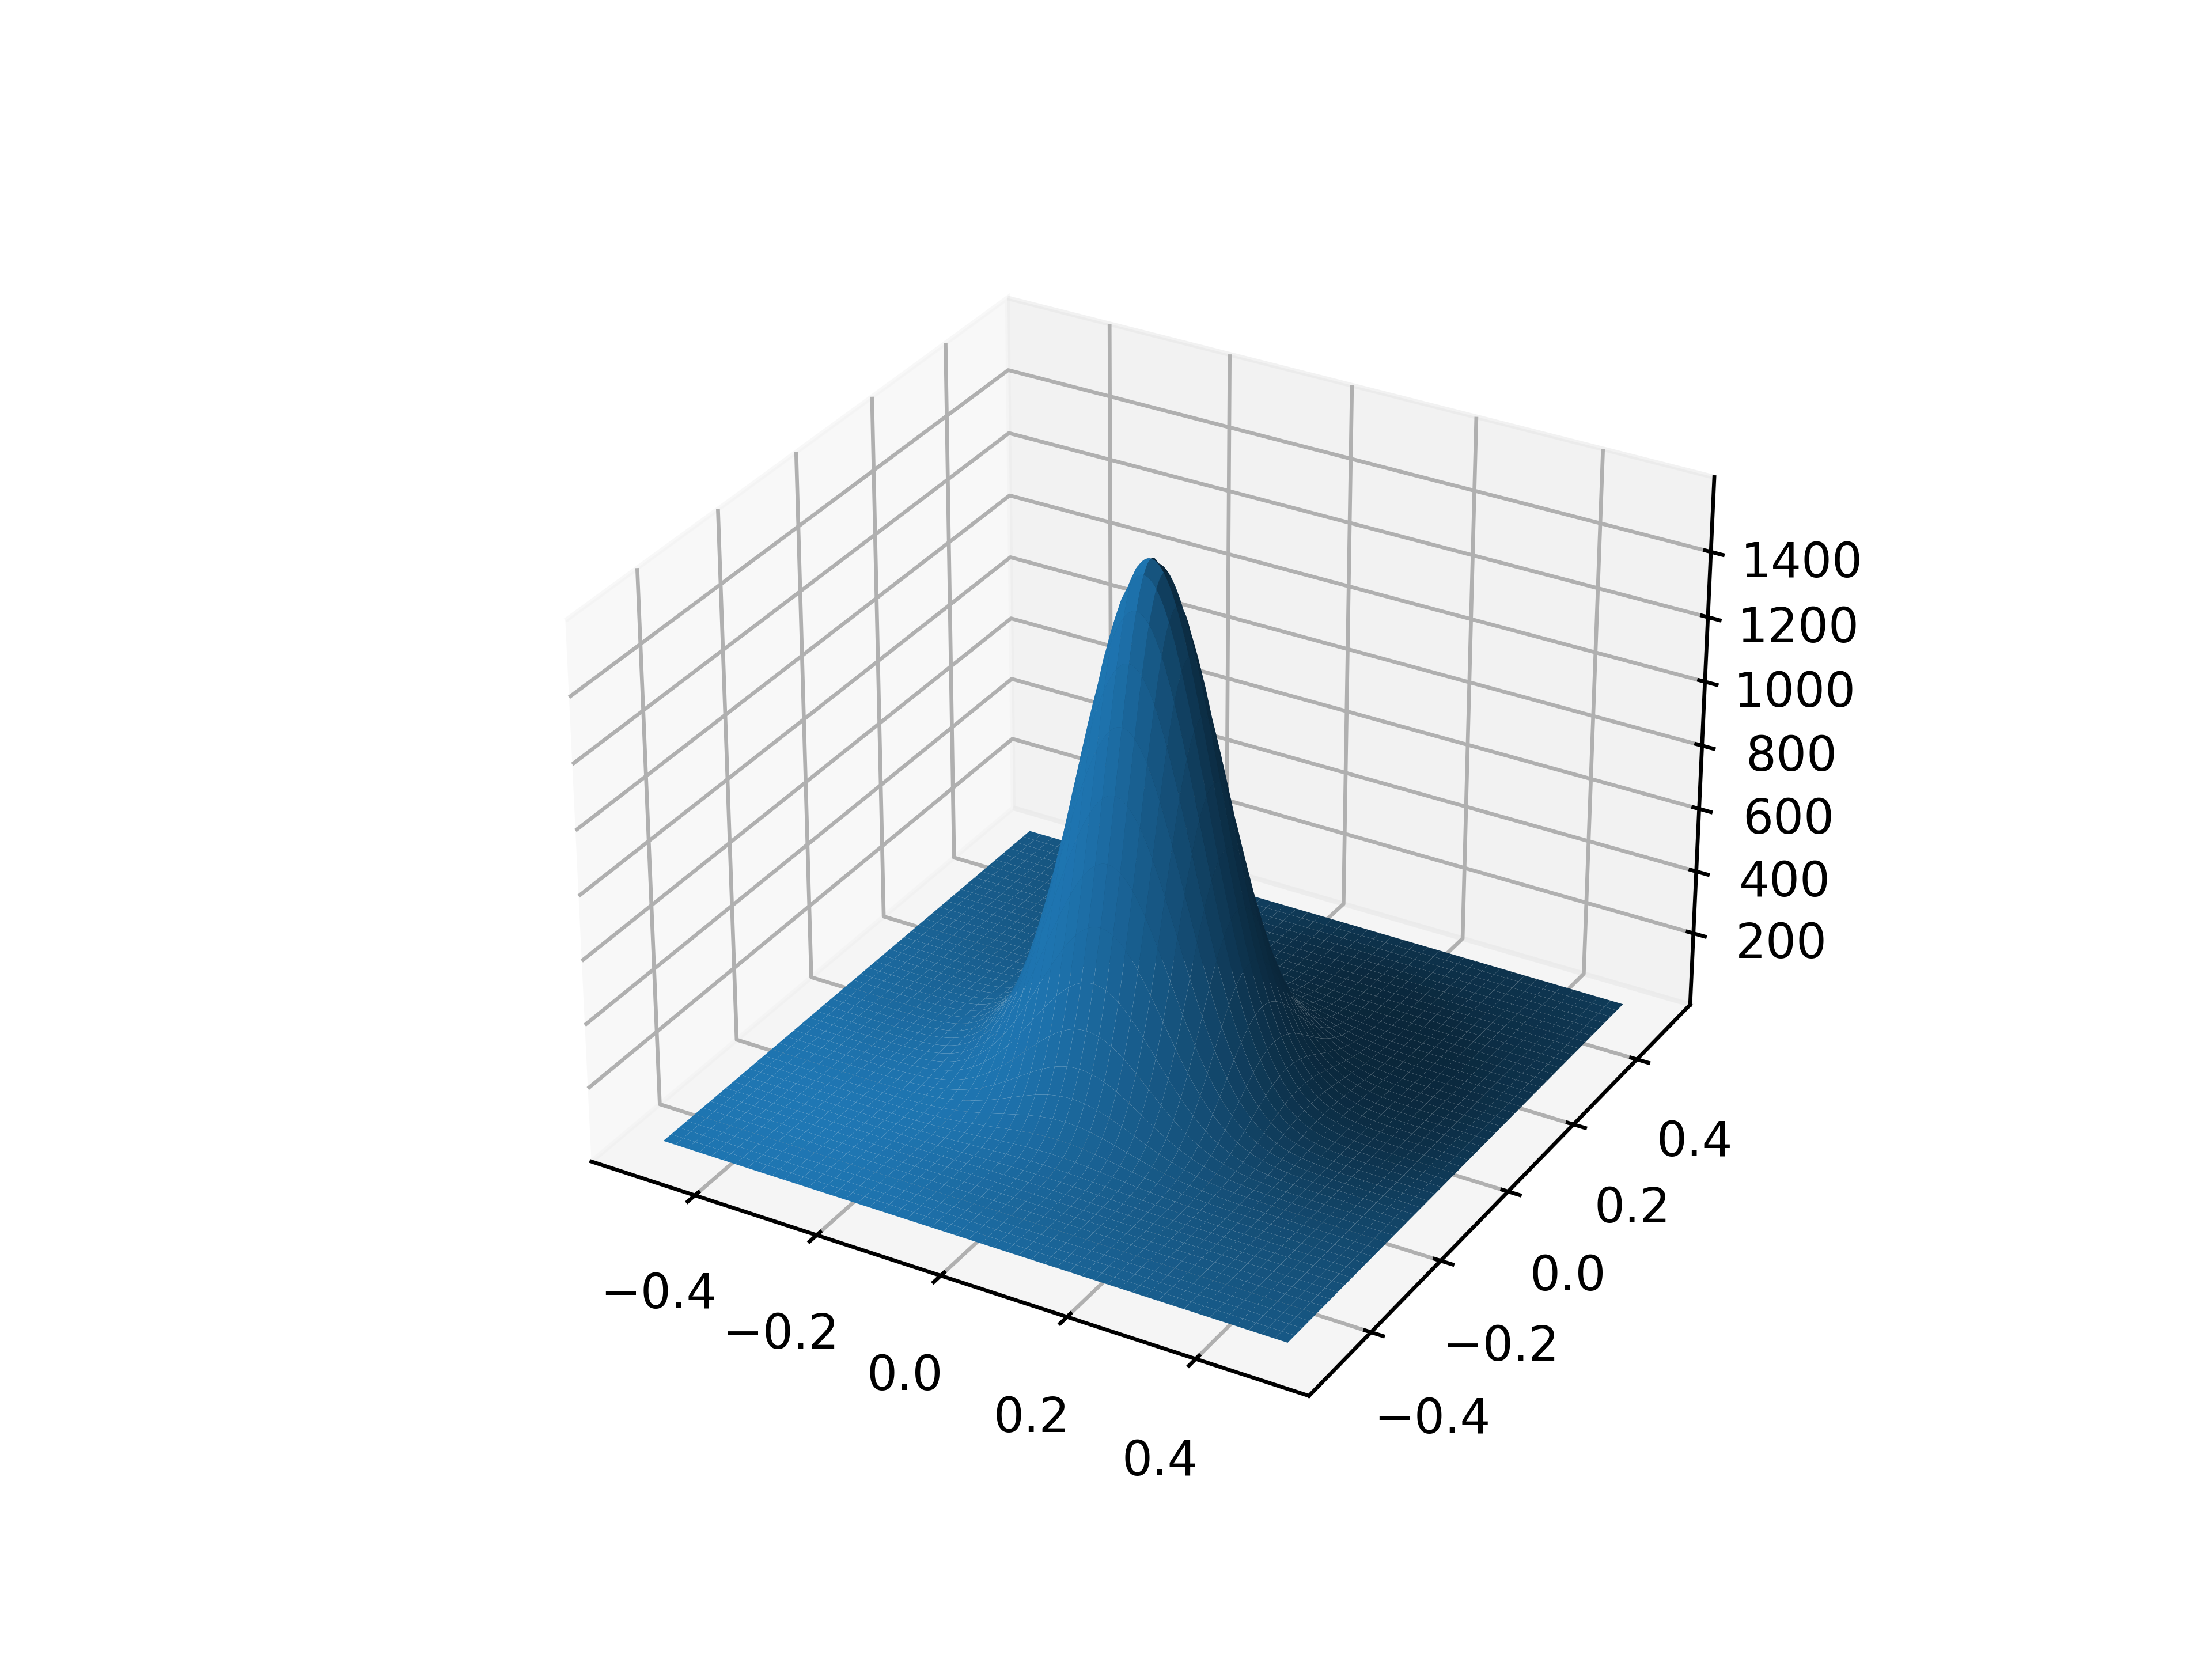
\includegraphics[scale=0.5, trim={1cm 1cm 1cm 1cm},clip]{figs/spike_example.png}
    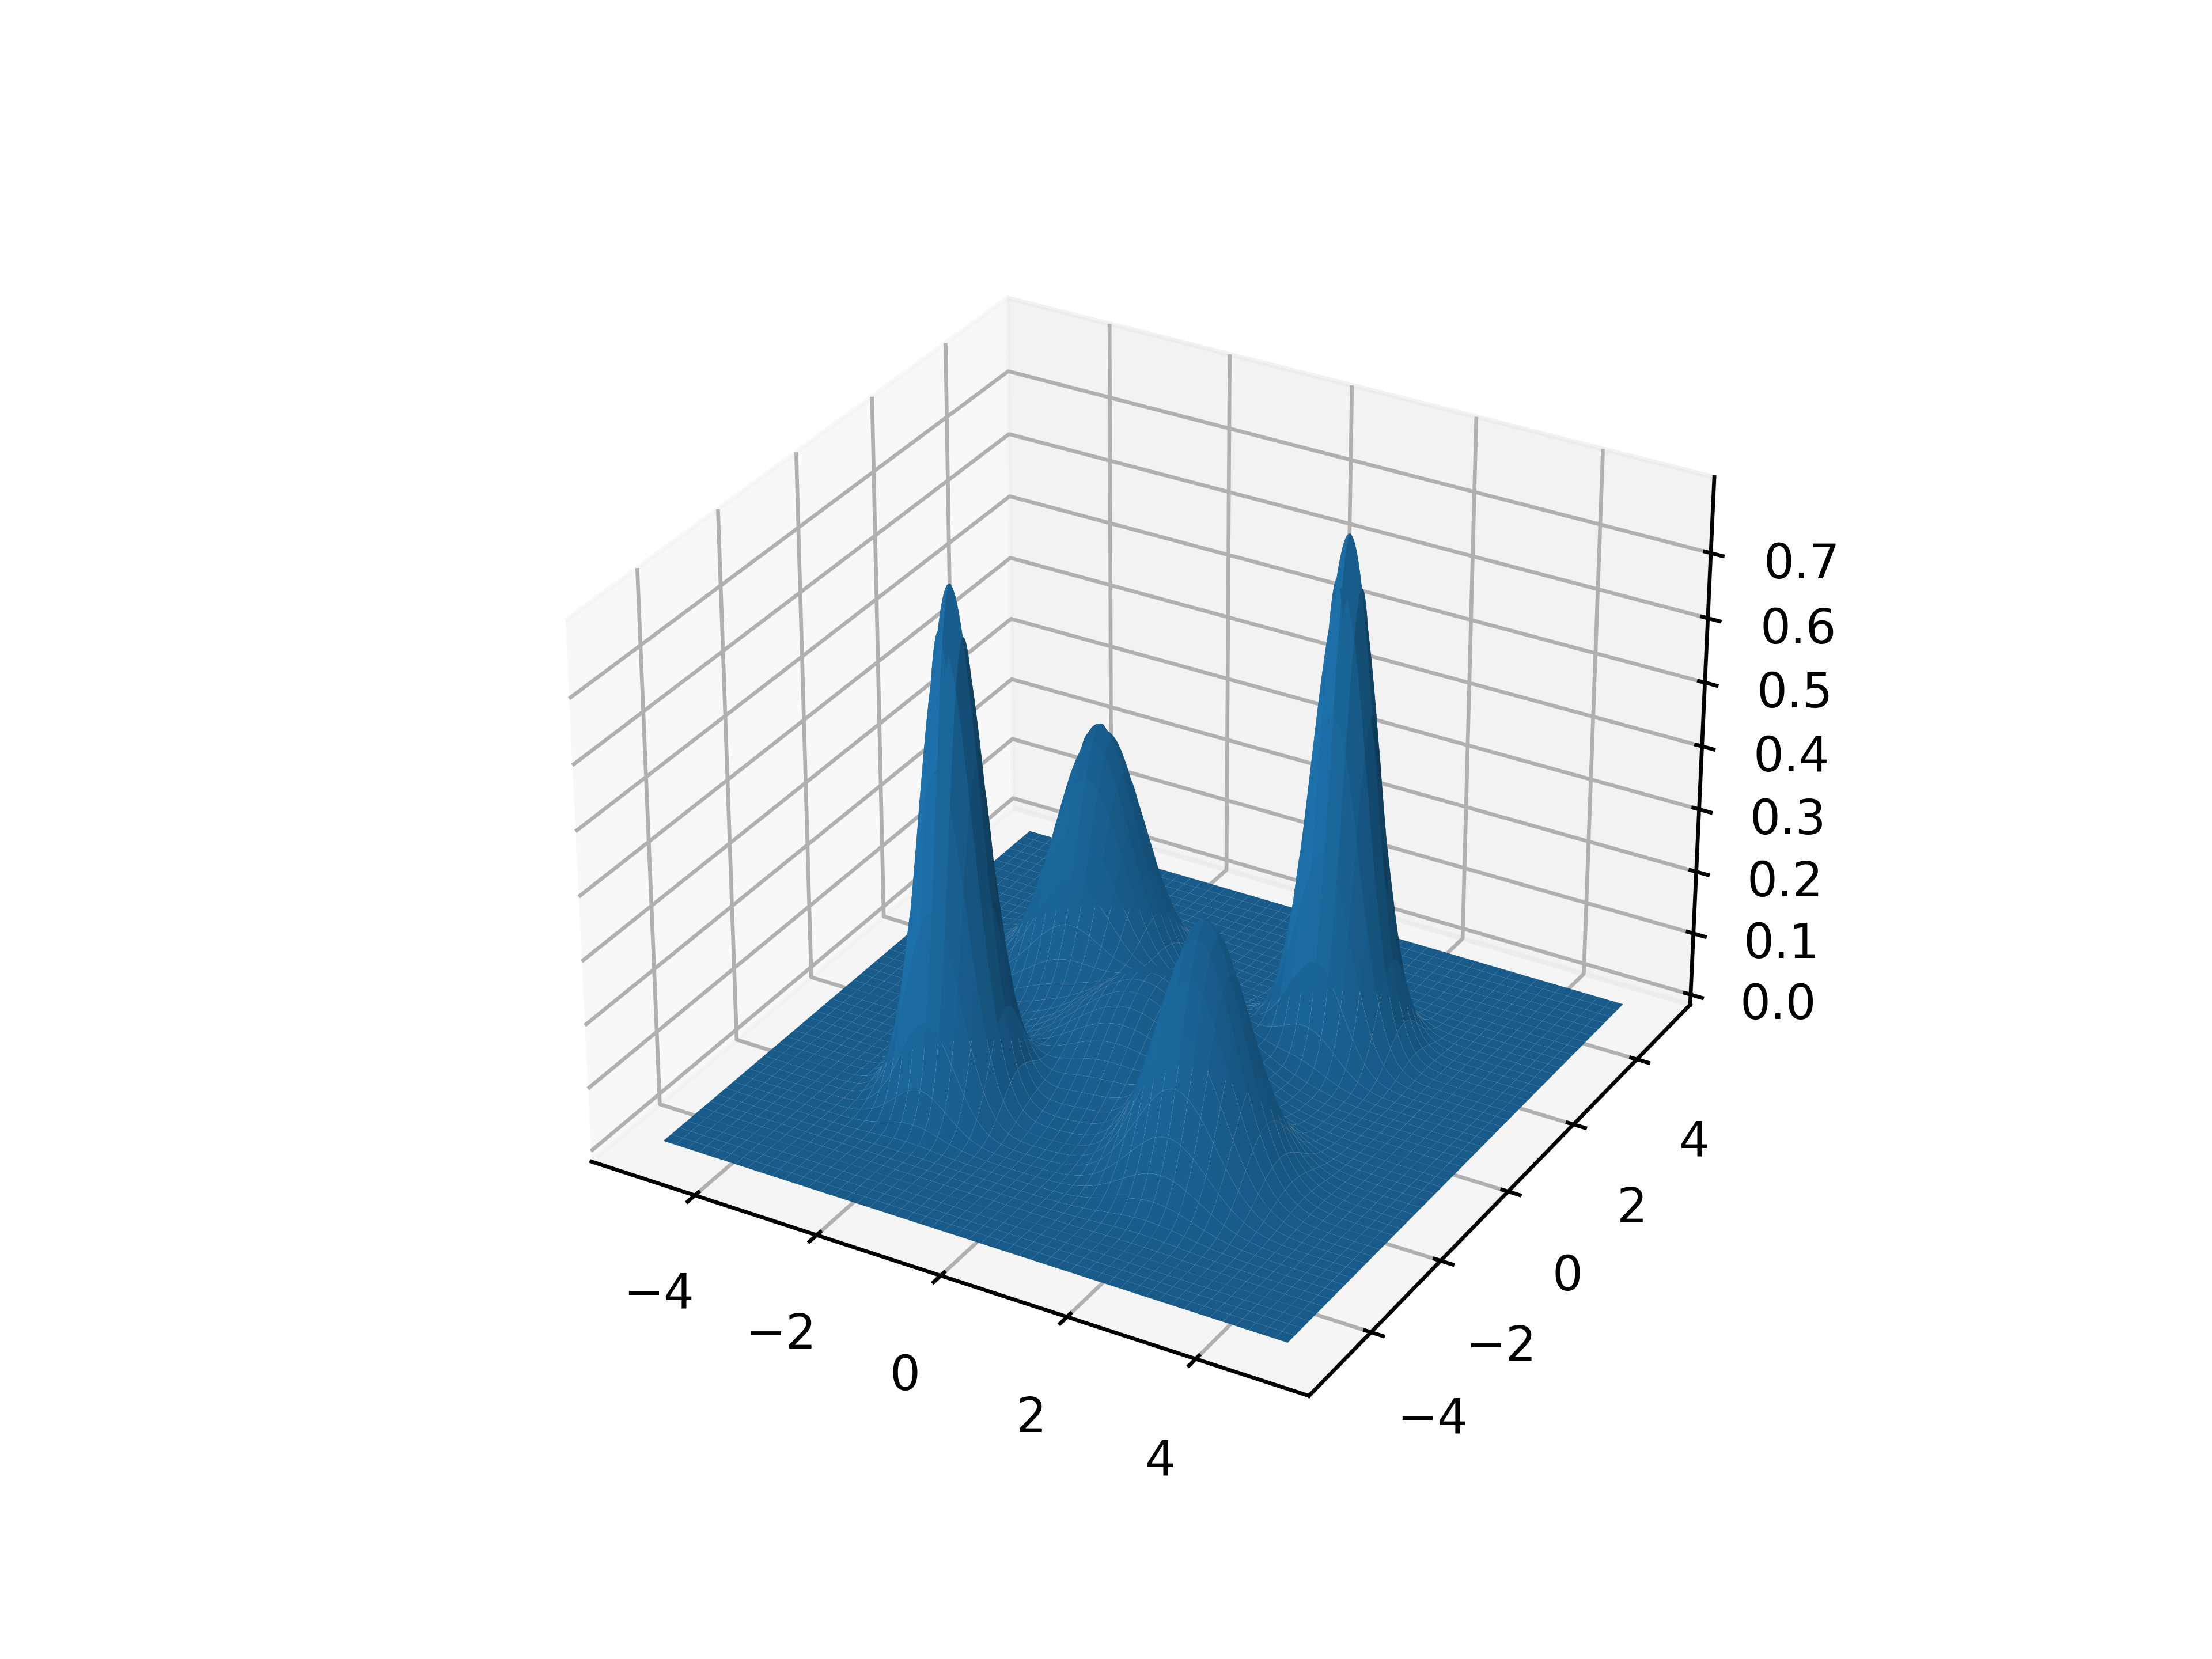
\includegraphics[scale=0.5, trim={1cm 1cm 1cm 1cm},clip]{figs/gauss_example.png}
    \label{fig:benchmark_examples}
    \caption{Plot of the 2D example problem likelihoods with the slab-and-spike on the left and the nonconcentric Gaussians on the right.}
\end{figure}

The spike-and-slab examples use a uniform prior on $[-0.5, 0.5]$ over all dimensions, while the nonconcentric Gaussians use a uniform prior on $[-5, 5]$.
Since the behaviour of Nested Sampling is heavily dependent on the method for LRPS used, I applied both standard Nested Sampling and the Barriers variant to each example problem with different LRPS methods.
The following LRPS approaches were used:
\begin{itemize}
    \item Metropolis Algorithm (with simple adaptive step size)
    \item HMC with reflection (only for standard Nested Sampling, with simple adaptive step size)
    \item HMC (only for Nested Sampling with Barriers, with simple adaptive step size)
    \item an optimal method for sampling inside an n-sphere (only for slab-and-spike examples)
\end{itemize}
Each configuration of example problem, algorithm and LRPS method was run 1000 times, with each run using 1000 live points and a stopping criterion of $\epsilon = 10^{-16}$.


\subsection{Influence of $t$ and $q_{\textrm{max}}$}

\chapter{Summary}

\clearpage
\printbibliography
\addcontentsline{toc}{chapter}{Bibliography}

\clearpage
\chapter*{Appendix}
\addcontentsline{toc}{chapter}{Appendix}
\subsection*{Proof: LRPS Samples' Prior Masses are Uniformly Distributed}
Let $\mathbb{T}$ be a random variable with $f_T(\theta) = \pi(\theta) \, \mathbbm{1}_{\{L(\theta)>L^*\}}(\theta)$.
Let $\mathbb{L} = L(\mathbb{T})$ and $\mathbb{M} = \mu(\mathbb{L})$.
$\mathbb{M}$ represents the prior masses, we want to prove that it follows a uniform distribution.
Because we are dealing with a likelihood-restricted prior, the uniform distribution is not on $[0,1]$, but on $[0, \mu(L^*)]$.
\begin{equation*}
    f_\mathbb{L}(\lambda) = \int_\Theta \delta(\lambda - L(\theta)) \, \pi(\theta) \, \mathbbm{1}_{\{L(\theta)>L^*\}}(\theta) \, d\theta,
\end{equation*}
Plugging the PDF-formula into the CDF:
\begin{align}
    F_\mathbb{L}(\lambda) &= \int_0^\lambda f_\mathbb{L}(\lambda') \, \mathbbm{1}_{\{L(\theta)>L^*\}}(\theta) \, d\lambda' \nonumber\\
    &= \int_0^\lambda \int_\Theta \pi(\theta) \, \mathbbm{1}_{\{L(\theta)>L^*\}}(\theta) \, \delta(\lambda' - L(\theta)) \, d\theta \, d\lambda' \nonumber\\
    &= \int_\Theta \int_0^\lambda \pi(\theta) \, \mathbbm{1}_{\{L(\theta)>L^*\}}(\theta) \, \delta(\lambda' - L(\theta)) \, d\lambda'\, d\theta \nonumber\\
    &= \int_\Theta \pi(\theta) \, \mathbbm{1}_{\{L(\theta)>L^*\}}(\theta) \int_0^\lambda \, \delta(\lambda' - L(\theta)) \, d\lambda' \, d\theta \nonumber\\
    &= \int_\Theta \pi(\theta) \, \mathbbm{1}_{\{L(\theta)>L^*\}}(\theta) \, \mathbbm{1}_{\{L(\theta) < \lambda\}}(\theta) \, d\theta \nonumber\\
    &= \int_{\{L^* < L(\theta) < \lambda\}} \pi(\theta)\, d\theta \label{eq:prior_mass_integral_appendix}\\
    &= \mu(L^*) - \mu(\lambda) \nonumber
\end{align}
See also the visualization for the last step in Figure \ref{fig:vis_prior_masses_lrps_appendix}.

$\mathbb{Y} = f(\mathbb{X})$ is uniform if $f$ is the CDF of $\mathbb{X}$ \cite[54]{casellaberger}.
This means that $\overline{\mathbb{M}} = \mu(L^*) - \mu(\mathbb{L})$ would be uniformly distributed on $[0,\mu(L^*)]$, since $\mu(L^*) - \mu(\lambda)$ is the CDF of $\mathbb{L}$.
And since $\mathbb{M}$'s values are simply the values of $\overline{\mathbb{M}}$ mirrored, $\mathbb{M}$ is also uniformly distributed.
\hfill $\qed$

\begin{figure}
    \centering
    \begin{tikzpicture}
        \begin{axis} [
            axis lines=center,
            xticklabel=\empty,
            yticklabel=\empty,
            xtick=\empty,
            ytick=\empty,
            xlabel=$\theta$,
            x label style={at={(axis description cs:0.53,-0.02)},anchor=north}
        ]
        \addplot[
            name path=A,
            domain=-0.5:6, 
            samples=200,
            color=blue
        ] { e^(-(x-3)^2) };
        \addplot[
            name path=B,
            domain=0:6, 
            samples=200,
            color=purple
        ] { 1/6 };
        \addplot[
            name path=C,
            dashed,
            domain=0:6, 
            samples=200,
            color=black
        ] { 0.8 };
        \addplot[
            name path=E,
            dashed,
            domain=0:6, 
            samples=200,
            color=black
        ] { 0.4 };
        \addplot[
            name path=D,
            domain=0:6,
            opacity=0
        ] {0};
        \draw[color=black, dashed] (axis cs:2.54, 0) -- (axis cs:2.54, 0.8);
        \draw[color=black, dashed] (axis cs:3.45, 0) -- (axis cs:3.45, 0.8);
        \draw[color=black, dashed] (axis cs:2.06, 0) -- (axis cs:2.06, 0.4);
        \draw[color=black, dashed] (axis cs:3.94, 0) -- (axis cs:3.94, 0.4);
        \addplot[ 
            color=gray,
            opacity=0.2, 
            ] fill between [
                of=B and D,
                soft clip={domain=2.06:2.54} 
        ];
        \addplot[ 
            color=gray,
            opacity=0.2, 
            ] fill between [
                of=B and D,
                soft clip={domain=3.45:3.94} 
        ];
        \node [color=black] at (axis cs:-0.3,0.81) {$\lambda$};
        \node [color=black] at (axis cs:-0.3,0.41) {$L^*$};
        \end{axis}
    \end{tikzpicture}
    \caption{Visualization of the integral in (\ref{eq:prior_mass_integral_appendix}). The shaded region is the integral, equivalent to $\mu(L^*) - \mu(\lambda)$.}
    \label{fig:vis_prior_masses_lrps_appendix}
\end{figure}

\chapter*{Declaration of Academic Integrity}
\footnotesize
1. I hereby confirm that this work — or in case of group work, the contribution for which I am
responsible and which I have clearly identified as such — is my own work and that I have not used
any sources or resources other than those referenced. 
I take responsibility for the quality of this text and its content and have ensured that all information and arguments provided are substantiated with or supported by appropriate academic sources. 
I have clearly identified and fully referenced any material such as text passages, thoughts, concepts or graphics that I have directly or indirectly copied from the work of others or my own previous work. 
Except where stated otherwise by reference or acknowledgement, the work presented is my own in terms of copyright.

2. I understand that this declaration also applies to generative AI tools which cannot be cited
(hereinafter referred to as ‘generative AI’).
I understand that the use of generative AI is not permitted unless the examiner has explicitly
authorized its use (Declaration of Permitted Resources).
Where the use of generative AI was permitted, I confirm that I have only used it as a resource and that this work is largely my own original work.
I take full responsibility for any AI-generated content I included in my work.
Where the use of generative AI was permitted to compose this work, I have acknowledged its use
in a separate appendix.
This appendix includes information about which AI tool was used or a detailed description of how it was used in accordance with the requirements specified in the examiner’s Declaration of Permitted Resources.
I have read and understood the requirements contained therein and any use of generative AI in this
work has been acknowledged accordingly (e.g. type, purpose and scope as well as specific
instructions on how to acknowledge its use).

3. I also confirm that this work has not been previously submitted in an identical or similar form to
any other examination authority in Germany or abroad, and that it has not been previously
published in German or any other language.

4. I am aware that any failure to observe the aforementioned points may lead to the imposition of
penalties in accordance with the relevant examination regulations.
In particular, this may include that my work will be classified as deception and marked as failed. Repeated or severe attempts to deceive may also lead to a temporary or permanent exclusion from further assessments in my degree programme.

\vspace{50pt}

Jena, 25.08.2022
\pagenumbering{gobble}

\end{document}
